\documentclass[double,12pt]{beavtex}

\usepackage{fancyhdr}
% link to section command
\newcommand{\HR}[1]{\hyperref[#1]{\ref{#1}}}

% for creating an index at end of document
\usepackage{imakeidx}
\makeindex[columns=1, title=Alphabetical Index]

% indexing commands
\newcommand{\bind}[1]{#1\index{#1}}
\newcommand{\iind}[1]{\textit{#1}\index{#1}}
\newcommand{\ind}[1]{#1\index{#1}}

\usepackage[hypertexnames=false]{hyperref}
\hypersetup{
    unicode=false,          % non-Latin characters in Acrobat’s bookmarks
    pdftoolbar=true,        % show Acrobat’s toolbar?
    pdfmenubar=true,        % show Acrobat’s menu?
    pdffitwindow=false,     % window fit to page when opened
    pdfstartview={FitH},    % fits the width of the page to the window
    pdftitle={Pommerenck Thesis},    % title
    pdfauthor={Jordan K. Pommerenck},     % author
    pdfsubject={Subject},   % subject of the document
    pdfcreator={Creator},   % creator of the document
    pdfproducer={Producer}, % producer of the document
    pdfkeywords={flat-histogram, Monte Carlo, Thesis}, % list of keywords
    pdfnewwindow=true,      % links in new PDF window
    colorlinks=true,       % false: boxed links; true: colored links
    linkcolor=black,          % color of internal links (change box color with linkbordercolor)
    citecolor=black,        % color of links to bibliography
    filecolor=magenta,      % color of file links
    urlcolor=cyan           % color of external links
}
%\usepackage{blindtext}
\usepackage[T1]{fontenc}
\usepackage[utf8]{inputenc}
\usepackage[document]{ragged2e}
% differential and partials package
\usepackage[thinc]{esdiff}
\usepackage{physics}
\newcommand{\D}[1]{\text{d}#1}
% the nth superscript package
\usepackage[super]{nth}

\usepackage{indentfirst}
\usepackage{graphicx}
\graphicspath{{../square-well/}{../ising/}{../gas-adsorption/figs/}}

\usepackage{caption}
\usepackage{float}
\usepackage{amsmath,amssymb}
\usepackage{nicefrac}

% Use more than one optional parameter in a new commands
\usepackage{xargs}
\usepackage[pdftex,dvipsnames]{xcolor}
\usepackage[colorinlistoftodos,prependcaption,textsize=normalsize]{todonotes}
\usepackage{mdframed}
\usepackage{braket}

% gas adsorption commands
\usepackage{subcaption}
\usepackage{url}
%
\usepackage[colorinlistoftodos,prependcaption,textsize=normalsize]{todonotes}

\newcommand{\addcite}{{\bf \color{red} []}}
\newcommand{\rvec}{\mathbf{r}}
\newcommand{\kvec}{\mathbf{k}}
\newcommand{\thetavec}{\boldsymbol \theta}
\newcommand\V{\Phi}
\newcommand\Vk{\tilde\Phi(\kvec)}
\newcommand\volume{V}
\newcommand\pfull{\ensuremath{p_{\text{full}}}}
\newcommand\pempty{\ensuremath{p_{\text{empty}}}}
\newcommand\mufull{\ensuremath{\mu_{\text{full}}}}
\newcommand\muempty{\ensuremath{\mu_{\text{empty}}}}
\newcommand\rhofull{\ensuremath{\rho_{\text{full}}}}
\newcommand\rhoempty{\ensuremath{\rho_{\text{empty}}}}
\newcommand\gst{\ensuremath{\Delta g_{st}}}

\newcommandx{\jordan}[2][1=inline]{\todo[linecolor=gray,backgroundcolor=gray!25,bordercolor=gray,#1]{\textbf{Jordan says:} #2} }
\newcommandx{\corysays}[2][1=inline]{\todo[linecolor=green,backgroundcolor=green!25,bordercolor=green,#1]{\textbf{Cory says:} #2} }

\newcommandx{\maybecut}[1]{\begin{mdframed}[backgroundcolor=cyan!24]\textbf{Maybe cut:} #1\end{mdframed} }

\newtheorem{limitation}{Limitation}

\renewcommand{\chaptername}{}

\title{Advancing Renewable Gas Storage using Flat-histogram Methods}
\author{Jordan K. Pommerenck}
\degree{Doctor of Philosophy}
\doctype{Dissertation}
\department{Physics}
\depttype{Department}
\depthead{Head}
\major{Physics}
\advisor{David Roundy}
\submitdate{June 8, 2020}
\commencementyear{2020}
\abstract{This work introduces the novel flat-histogram Monte Carlo (MC) method
stochastic approximation with a dynamic update factor (SAD) and explores the
convergence properties of a variety of related weight-based MC methods. The new
method is applied to a number of physical `test’ systems including the 2D Ising
model, a square-well fluid, and a 31 atom Lennard-Jones cluster. We find that
SAD performs robustly on all of the systems. Also, SAD efficiently samples the
entire energy space defined by a chosen temperature range (rather than using
unphysical parameters). Additionally, we develop a theoretical upper bound for
gas adsorption and delivery in porous materials and compare the upper bound with
experimental data.
A driving motivation for developing the novel Monte Carlo method SAD is to
provide a simulation method for computing the thermodynamic properties of
porous materials. By computationally determining a materials deliverable
capacity, researchers save countless development and experimental hours. In
particular, this body of research heavily contributes to enabling light-vehicle
gas storage applications.}
\acknowledgements{I gratefully acknowledge my graduate advisor David Roundy for his constant
support and guidance throughout my research. His breadth of knowledge and
hands-off approach to advising have tremendously helped my development as an
independent scientific researcher. I express thanks to my entire graduate
committee: David McIntyre, Davide Lazzati, Yun-Shik Lee, and graduate council
representative Chih-hung (Alex) Chang. I would like to acknowledge the many
outstanding undergraduate and graduate students that have positively impacted
me personally and professionally while at Oregon State University. Finally, I
would like to thank my parents for their unconditional support throughout my
Ph.D. research.}
\contributors{Michael A. Perlin worked on much of the early C{}\verb!++! codebase. This
codebase was used primarily in the early study of many of the MC methods before
switching to RUST. In addition, he helped in the editing phase during the
preparation of the first manuscript \emph{Stochastic approximation Monte Carlo
with a dynamic update factor}. Tanner T. Simpson performed many of the early
simulations for the flat-histogram methods using the C{}\verb!++! codebase. He
also developed using Python some of the plotting scripts that allowed the saved
C{}\verb!++! data to be visualized. In addition, he helped in the editing phase
during the preparation of the first manuscript \emph{Stochastic approximation
Monte Carlo with a dynamic update factor}. Cory M. Simon collaborated together
with us on the third manuscript \emph{An upper bound to gas delivery via
pressure-swing adsorption in nanoporous materials}. He contributed
significantly to the introduction section of the paper and helped in the
editing phase throughout preparation. In addition, he designed the first figure
in the paper and the first figure in the supplemental to the paper.}

\begin{document}

\maketitle

\mainmatter

\setlength\parindent{24pt}
\begingroup
\let\clearpage\relax
\begin{center}
\large
Advancing Renewable Gas Storage using Flat-histogram Methods
\normalsize
\end{center}
\chapter{Introduction}
Monte Carlo methods are a powerful simulation tool that allow scientists to explore properties of systems that may otherwise by inaccessible via experimental methods. Monte Carlo methods can be used to solve a variety of physical problems yielding insight into statistical averages due to random processes. During the last two decades considerable research has been done on developing and refining flat-histogram Monte Carlo methods.  These Monte Carlo (MC) methods are capable of exploring all of the energy phase space for all given temperatures in a \emph{single} simulation. In this work, we first outline the necessary statistical mechanics background. We provide a description of MC methods and flat-histogram methods, as well as, our newly developed method SAD (stochastic approximation Monte Carlo with a dynamic update factor). We discuss physics rich test systems that can be used to explore the convergence and statistical properties of our newly developed method SAD. 

A driving motivation for developing novel Monte Carlo methods that have physically based tunable parameters is to provide simulation methods for exploring metal-organic frameworks (MOFs). In this work, we examine MOFs and
their application to gas storage and delivery. We formulate a theoretical upper
bound on the maximum amount of gas that can be stored and released at different
pressures. We propose SAD as a powerful method for examining thermodynamic properties for MOFs.  We lay a groundwork for 2D SAD which would be able to compute isotherms for any given MOF thereby providing a powerful way for researchers to determine a MOF's suitability for gas storage applications.

In the following chapters, we follow the manuscript outline with each chapter corresponding to our published or submitted research on the SAD method applied to various physical systems and our work on establishing a theoretical upper bound on gas storage and delivery for MOFs.

\section{Micro-Canonical Ensemble}\label{micro}
A statistical ensemble is defined as a probability distribution $\mathcal{P}\left(\Omega\right)$ for the state of the system.
The micro-canonical\index{ensemble!micro-canonical} is a representation for a system $\Gamma$ that is determined by a fixed number\index{extensive!number $N$} of particles $N$ (and fixed components $\sum N_i$ for a multi-component system), a fixed volume\index{extensive!volume $V$} $V$, and a fixed energy\index{extensive!energy $E$} $E$. All possible states for the system $\Gamma\left(N,V,E\right)$ have the same number of particles, energy, and volume due to the system being in isolation from any external environment.
The micro-canonical ensemble\index{ensemble!micro-canonical} is for this reason also known as the $NVE$ ensemble as the micro-states depend on the \ind{extensive} macroscopic details.

The probability $\mathcal{P}$ of selecting a micro-state at random for a given range of energies centered about $E$ is given by
\begin{align}
    \mathcal{P} = \frac{1}{\Omega(E)}
\end{align}
where $\Omega(E)$ is the number of micro-states in the system $\Gamma(E)$.

\subsection{Definition of Entropy $S(E)$}\label{entropy}
The entropy $S(E)$ can be defined for any given system $\Gamma$ with discrete energy states using one of the most important formulae in physics:
\begin{align}\label{sdos}
    S(E,V,N) \equiv k_B \ln\Omega(E,V,N)
\end{align}
where the entropy is defined as the logarithm of the density of states and $k_B$ is the Boltzmann constant. An important aspect of this definition in terms of logarithms is that the entropy for multiple isolated systems is additive.
\begin{align}
    S(E_1,E_2) &= k_B \ln(\Omega(E_1)\Omega_2(E_2)) \\
    &= k_B \left( \Omega_1(E_1) + \Omega_2(E_2)\right) \\
    &= k_B \left( S_1(E_1) + S_2(E_2)\right)
\end{align}
From the \nth{1} law of thermodynamics, the system temperature can be written in terms of the density of states by referring to Eq.~\HR{sdos}.
\begin{align}
    T = \left(\diff{S(E)}{E}\right)_V = \frac{k_B}{\Omega(E)}\left(\diff{\Omega(E)}{E}\right)_V
\end{align}
The relationship between entropy $S(E)$, $\Omega(E)$, and $T$ will be discussed in further depth in Section~\HR{laws}.

\subsection{The Laws of Thermodynamics and $S(E)$}\label{laws}
The \nth{1} law of thermodynamics states that for an isolated system $\Gamma$, the total internal energy is equal to the sum of the heat $Q$ and work $W$ done.
\begin{align}
    \D{U} = \D{Q} + \D{W}
\end{align}
The \nth{1} law follows directly from conservation of energy. The thermodynamic identity states that for any infinitesimal change in the system and fixed number of particles $N$, the internal energy can be written in terms of the entropy.
\begin{align}
    \D{U} =  T\D{S} - p\D{V} \\
    T = \left(\diff{U}{S}\right)_V
\end{align}

The \nth{2} law of thermodynamics states that for any isolated system $\Gamma$ the entropy $S(E) \geq 0$. The heat of the system can also be related to the entropy using the relation:
\begin{align}
    \delta Q = T\delta S
\end{align}
The relationship between heat and entropy for a system is invaluable for the \nth{1} law to relate the conjugate variables T, $S(E)$, and $U(E)$.

\section{Canonical Ensemble}
The Canonical ensemble is a representation for a system $\Gamma$ that is determined by a fixed number of particles $N$ (and fixed components $\sum N_i$ for a multi-component system), a fixed volume $V$, and a fixed temperature $T$. All possible states for the system $\Gamma\left(N,V,T\right)$ have the same number of particles, energy, and temperature due to the system being in thermal equilibrium with a heat bath.
The canonical ensemble is for this reason also known as the $NVT$ ensemble.

The probability $\mathcal{P}$ of selecting a given micro-state at random is
\begin{align}
    \mathcal{P} = e^{\nicefrac{F-E}{k_BT}}
\end{align}
where $F\left(N,V,T\right)$ is the free energy of the system $\Gamma$ and will be discussed in detail in section~\HR{potentials}.



\subsection{Boltzmann Factor and Partition Function}
In statistical thermodynamics $\beta$ is defined as the coldness or the reciprocal of the temperature.
\begin{align}
    \beta = \frac{1}{k_BT} = \frac{1}{k_B}
\end{align}
where $k_B$ is the Boltzmann constant. The partition function for a canonical ensemble can then be written in terms of the Boltzmann factor where $E$ is the total energy of the system in the respective microstate at index $i$.
\begin{align}
    Z = \sum_i e^{-\beta E_i}
\end{align}

\subsection{Thermodynamic Potentials}\label{potentials}
Thermodynamic potentials describe a given thermodynamic state of a given system and
have units of energy $k_BT$. In this section, we will discuss five common thermodynamic potentials and how they are mathematically related through Maxwell relations.
While the internal energy $U(E)$ has been briefly mentioned in section~\HR{laws}, we outline in detail the relationship between the state variables.
\begin{align}
    \D{U(S,V,N)} = T\D{S}-p\D{V}+\mu\D{N}
\end{align}
We can write the temperature $T$, pressure $p$, and chemical potential $\mu$ in terms of derivatives of state variables.
\begin{align}\label{maxU}
    T = \left( \pdv{U}{S}\right )_{V,N}  \quad\quad 
    p = -\left( \pdv{U}{V}\right )_{S,N}  \quad\quad 
    \mu = \left( \pdv{U}{N}\right )_{S,V}  \quad
\end{align}
The Helmholtz free energy $F(T,V,N)$ can be written as follows:
\begin{align}
    \D{F(T,V,N)} = \D{(U-TS)} = -S\D{T}-p\D{V}+\mu\D{N}
\end{align}
We can write the entropy $S$, pressure $p$, and chemical potential $\mu$ in terms of derivatives of state variables.
\begin{align}\label{maxF}
    S = \left( \pdv{F}{T}\right )_{V,N}  \quad\quad 
    p = -\left( \pdv{F}{V}\right )_{T,N}  \quad\quad 
    \mu = \left( \pdv{F}{N}\right )_{T,V}  \quad
\end{align}
The Enthalpy $H(S,p,N)$ can be written as follows:
\begin{align}
    \D{H(S,p,N)} = \D{(U+pV)} = -T\D{S}+V\D{p}+\mu\D{N}
\end{align}
We can write the temperature $T$, volume $V$, and chemical potential $\mu$ in terms of derivatives of state variables.
\begin{align}\label{maxH}
    T = \left( \pdv{H}{S}\right )_{p,N}  \quad\quad 
    V = -\left( \pdv{H}{p}\right )_{S,N}  \quad\quad 
    \mu = \left( \pdv{H}{N}\right )_{S,p}  \quad
\end{align}
The Gibbs free energy $G(T,p,N)$ can be written as follows:
\begin{align}
    \D{G(T,p,N)} = \D{(U+pV-TS)} = -S\D{T}+V\D{p}+\mu\D{N}
\end{align}
We can write the entropy $S$, volume $V$, and chemical potential $\mu$ in terms of derivatives of state variables.
\begin{align}\label{maxG}
    S = \left( \pdv{G}{T}\right )_{p,N}  \quad\quad 
    V = -\left( \pdv{G}{p}\right )_{T,N}  \quad\quad 
    \mu = \left( \pdv{G}{N}\right )_{T,p}  \quad
\end{align}

\subsection{Maxwell Relations}\label{maxwell}
Maxwell's relations are second derivative equalities that relate important thermodynamic variables. Maxwell relations are an extension of the Schwarz theorem which states that the order of differentiation is irrelevant.
\begin{align}
    \pdv{}{\theta}\left(\pdv{\Theta}{\phi}\right)=\pdv{}{\phi}\left(\pdv{\Theta}{\theta}\right)
\end{align}
From this theorem and Section~\HR{potentials}, we can derive the most common of Maxwell's relations. The relation involving internal energy $U\left(S,V,N\right)$ relates the natural variables of pressure $p$ and temperature $T$ and can be derived using Equation~\ref{maxU}.
\begin{align}
    \left( {\pdv{U}{S}{V}} \right )_{N} = \left( \pdv{T}{V}\right )_{S,N} = - \left( \pdv{p}{S}\right )_{V,N}
\end{align}
The relation involving the Helmholtz free energy $F\left(T,V,N\right)$ relates the natural variables of entropy $S$ and pressure $p$ and can be derived using Equation~\ref{maxF}.
\begin{align}
    \left( {\pdv{F}{T}{V}} \right )_{N} = \left( \pdv{S}{V}\right )_{T,N} = \left( \pdv{p}{T}\right )_{V,N}
\end{align}
The relation involving the Enthalpy $H\left(S,p,N\right)$ relates the natural variables of temperature $T$ and volume $V$ and can be derived using Equation~\ref{maxH}.
\begin{align}
    \left( {\pdv{H}{S}{p}} \right )_{N} = \left( \pdv{T}{p}\right )_{S,N} =  \left( \pdv{V}{S}\right )_{p,N}
\end{align}
The relation involving the Gibbs free energy $G\left(T,p,N\right)$ relates the natural variables of entropy $S$ and volume $V$ and can be derived using Equation~\ref{maxG}.
\begin{align}
    \left( {\pdv{G}{T}{p}} \right )_{N} = -\left( \pdv{S}{p}\right )_{T,N} = - \left( \pdv{V}{T}\right )_{p,N}
\end{align}

\subsection{Thermodynamic Properties}\label{thermoprop}
The Maxwell relations from Section~\HR{maxwell} can be written in terms of thermodynamic properties of the material.  The isochoric heat capacity $C_V$ of a given material is defined as the amount of heat necessary to raise the temperature by a given amount.
\begin{align}
    C_V = \left(\pdv{U}{S}\right )_{V,N}\left( \pdv{S}{T} \right )_{V,N} = \frac{1}{T}\left(\pdv{S}{T}\right )_{V,N}
\end{align}
The isobaric heat capacity $C_p$, which is always greater than or equal to $C_V$ according to the Mayer relation, can also be written in terms of the entropy $S$ and temperature $T$ of the system.
\begin{align}
    C_p = \left(\pdv{U}{S}\right )_{V,N}\left( \pdv{S}{T} \right )_{p,N} = T\left(\pdv{S}{T}\right )_{p,N}
\end{align}
The Mayer relation gives the difference of the isobaric and isochoric heat capacities in terms of the thermal expansion coefficient and the isothermal compressibility.
\begin{align}
    C_p - C_V = VT\frac{\alpha^2}{\kappa_T}
\end{align}
The isobaric coefficient of thermal expansion determines to what extent a given material will deform as a result of a change in temperature.
\begin{align}
    \alpha_p = \frac{1}{V}\left( \pdv{V}{T} \right )_{p,N}
\end{align}
Similarly, the isochoric coefficient of thermal expansion can be written as the following:
\begin{align}
    \alpha_V = \frac{1}{p}\left( \pdv{p}{T} \right )_{V,N}
\end{align}
The compressibility determines to what extent a given material will change volume based on the pressure applied to the system.  The isothermal compressibility can be written in terms of the following:
\begin{align}
    \kappa_T = -\frac{1}{V}\left( \pdv{V}{p} \right )_{T,N}
\end{align}
Similarly, the isentropic compressibility can be written as the following:
\begin{align}
    \kappa_S = -\frac{1}{V}\left( \pdv{V}{p} \right )_{S,N}
\end{align}
A major driving force behind introducing the concepts of thermal expansion and compressibility is to right complex derivatives in terms of these parameters. The internal energy derivative and entropy derivative can be written in terms of both the isothermal compressibility and the thermal coefficient of expansion.
\begin{align}
    \left( \pdv{U}{p} \right )_{V,N} = \frac{\kappa_T C_p}{\alpha} - \alpha TV \quad\quad
    \left( \pdv{S}{p} \right )_{V,N} = \frac{\kappa_T C_p}{\alpha T} + \alpha V
\end{align}
Additionally, the enthalpy derivatives can be written in terms of both the isothermal compressibility and the thermal coefficient of expansion.
\begin{align}
    \left( \pdv{H}{T} \right )_{V,N} = C_p + \frac{\alpha V}{\kappa_T}\left(1-\alpha T\right) \quad\quad
    \left( \pdv{H}{p} \right )_{V,N} = \frac{\kappa_T C_p}{\alpha} + V\left(1-\alpha T\right)
\end{align}
Finally, the Gibbs free energy derivatives can be written in terms of the isothermal compressibility, the thermal coefficient of expansion, and the entropy.
\begin{align}
    \left( \pdv{G}{T} \right )_{V,N} = \frac{\alpha V}{\kappa_T}-S \quad\quad
    \left( \pdv{G}{p} \right )_{V,N} = V-\frac{\kappa_T S}{\alpha}
\end{align}

\section{Grand Canonical Ensemble}
The grand canonical ensemble is a representation for a system $\Gamma$ that is determined by a fixed chemical potential $\mu$, a fixed volume $V$, and a fixed temperature $T$. All possible states for the system $\Gamma\left(\mu,V,T\right)$ have the same chemical potential, volume, and temperature due to the system being in thermal and chemical equilibrium with a given resevoir.
The grand canonical ensemble is for this reason also known as the $\mu VT$ ensemble.

The probability $\mathcal{P}$ of selecting a given micro-state at random is
\begin{align}
    \mathcal{P} = e^{\nicefrac{\Phi + \mu N-E}{k_BT}}
\end{align}
where $\Phi\left(\mu,V,T\right)$ is the grand potential of the system $\Gamma$. The grand potential is often referred to as the Landau potential and written:
\begin{align}
    \Phi \equiv F -\mu N = U - TS -\mu N
\end{align}

\subsection{Chemical Potential $\mu$}
The chemical potential $\mu$ of a given system $\Gamma$ is representative of the energy that can be gained or lost due (often because of a phase transition) to a change in the conjugate variable particle number $N$. Analogous to potential energy, higher chemical potential drives particles to lower potential (thereby usually changing the particle number). The chemical potential $\mu_i$ of species $i$ can be represented using a variety of free energies (all of which are equivalent but not necessarily useful for any given experiment).
\begin{align}
    \mu_i = \left( \pdv{G}{N_i}\right )_{T,P,N_{j \neq i}}  \quad
    \mu_i = \left( \pdv{H}{N_i}\right )_{S,P,N_{j \neq i}}  \quad
    \mu_i = \left( \pdv{F}{N_i}\right )_{T,V,N_{j \neq i}}  
\end{align}

\subsection{Grand Potential and Thermodynamic Quantities}
A variety of important thermodynamic quantities can be written in terms of the grand potential. In differential form, the grand potential can be written as the following (for a single component system $\Gamma$):
\begin{align}
    \D{\Phi(\mu,V,T)} = -S\D{T}-p\D{V}-N\D{\mu}
\end{align}
The number $N$, pressure $p$, and Gibbs entropy $S$ can be written in terms of the grand potential.
\begin{align}
    N = -\left( \pdv{\Phi}{\mu}\right )_{T,V}  \quad
    p = -\left( \pdv{\Phi}{V}\right )_{T,\mu}  \quad
    S = -\left( \pdv{\Phi}{T}\right )_{V, \mu} 
\end{align}


\section{Monte Carlo Simulation}\label{monte}
Experiment and simulation blend together to help form a more complete understanding of our knowledge of how the universe works. Computational `experiments' such as Monte Carlo methods aid in this understanding by allowing scientists to explore system configurations that are not easily accessible to traditional experiment.

In the field of statistical physics, Monte Carlo methods are used to determine equilibrium 
properties (thermal averages) of multi-particle systems.  A number of Monte Carlo simulations 
have been developed over the last century. Some of these methods are completely unique while 
others are more sophisticated variants of an original method. All of the methods share a number 
of similarities including picking random moves (we will discuss this process in Section~\HR{rng}) and determining the acceptance or rejection of a 
move based on a probability distribution. They differ primarily in how they explore phase space 
and thus compute thermodynamic properties such as the density of states $\Omega(E)$. The accuracy of any MC simulation depends on the details of how the system is `explored'. To reduce the error 
in simulation one can in principle simply continue to allow the simulation more time to explore 
phase space.

The motivation for new research into developing MC methods stems from the desire to solve ever-increasingly complex physical problems in a faster simulation time. Many of the originally developed MC methods are unable to effectively explore the complex phase space of real (and even many test) systems. Flat-histogram methods (introduced in Section~\HR{fhm}) are able to explore all energies and temperatures in a `single' simulation. In addition, they are able to explore complex energy landscapes without getting `stuck' (either never converging or converging at such a slow rate as to not practically converge). Many of these flat-histogram methods also have proven convergence on the statistical error thus guaranteeing convergence.
In the following sections, we will discuss a number of MC methods including importance sampling canonical methods, and flat-histogram methods leading up to our method SAD introduced in this work discussed in Section~\HR{fhm}.

\subsection{Random Number Generation}\label{rng}

Since Monte Carlo moves are inherently stochastic in nature, it is imperative that any useful random number generator be fast and ideally non-deterministic. In practice, pseudo-random number generators (PRNGs) are used in order to generate the fast random streams although they are deterministic. In order for a PRNG to be acceptable for use in Monte Carlo simulation it must meet certain criteria~\cite{sawilowsky2003you}. First, the PRNG must have a long `period' before repeating values. Poor PRNGs (that is ones with short periods) can lead to systematic error in Monte Carlo simulations~\cite{ferrenberg1992monte, plascak2002cluster, ossola2004systematic}.
Second, the PRNG must actually be able to pass certain statistical tests such as implemented in the TestU01 library~\cite{l2007testu01}.

There are a variety of PRNGs each with benefits and few without some form of drawback. We detail some of the well known PRNGs here. Linear congruential generators (LCGs) have a very fast time performance and are straightforward to program (in terms of size and complexity). Unfortunately, LCGs have multiple issues regarding the generated random number statistical quality~\cite{coddington1994analysis, barry1996recommendations}. While the period of the PRNG can be made acceptable by using 64-bit integers, the statistical correlations remain. Other PRNGs are the belong to the shift-register family (Xorshift RNGs). Like the LCG family, the shift-register RNGs fail many statistical tests~\cite{panneton2005xorshift} and are therefore often considered unacceptable for use in Monte Carlo simulations.

In our works, we use the \textbf{Xoroshiro128+} RNG which is named after its logical operations (XOR $\xrightarrow{}$ rotate $\xrightarrow{}$ shift $\xrightarrow{}$ rotate). The RNG has ultra-fast speed 0.72 $\nicefrac{\text{ns}}{\text{64-bits}}$ and incredible statistical quality~\cite{blackman2018scrambled}.

\subsection{Canonical Monte Carlo}\label{cmc}
In this section, we introduce canonical Monte Carlo and how it relates to flat-histogram methods introduced in Section~\HR{fhm}. The first importance sampling method developed was the famous Metropolis method~\cite{metropolis1953equation}.  The method works by choosing an initial state for the system $\Gamma$. Next, a random site $\Gamma_i$ is chosen and a move is proposed that will result in an energy change $\Delta E$ if accepted. The acceptance of the move is determined by whether a random number chosen on a range from zero to one is less than a Boltzmann factor. The process of moves and random number generation is repeated until some termination condition is met. This canonical method performs calculations at a fixed temperature $T$ only. Re-weighting can extrapolate in the vicinity of the simulated temperature, but this approach is limited. Another limitation of canonical Monte Carlo is that for complex energy landscapes and/or large systems the simulation can undergo a phenomena known as `critical slowing down' as the simulation will never or almost never visit the ground state energy $E_{\min}$~\cite{berg2000introduction}. These limitations are what drive the need for methods that can avoid getting `stuck' and that can simulate all temperatures in a single simulation.

\subsection{Flat-Histogram Methods}\label{fhm}
The goal of flat-histogram methods (also called \emph{broad-histogram}
or \emph{multicanonical} methods) is to simulate each energy with
similar accuracy.  In this way, they can accurately determine the density of states
over a broad range of energies and thus determine the thermodynamic
quantities such as heat capacity or internal energy
over a broad range of temperatures.
Properties that require more information, such as a spatial
correlation function or a response function, can still be computed
for any temperature, provided statistics are collected for each
individual energy, which can then be reweighted for any
temperature~\cite{panagiotopoulos1998phase, panagiotopoulos2000monte,
errington2003direct}.
All the flat-histogram Monte Carlo methods begin with randomly chosen
`moves' which change the state of the system and must satisfy
detailed balance.  All of the tested algorithms differ in how they determine the
probability of accepting a move and in what additional statistics must
be collected in order to decide on that probability.
Flat-histogram methods calculate the density of states $D(E)$ for a discrete set
of energies~\cite{wang2001determining, dayal2004performance, troyer2003flat,
trebst2004optimizing}. Therefore, energy binning becomes an important
consideration for systems with a continuum of possible energies.  Energy bins
are typically of uniform size for the entire energy
continuum~\cite{fasnacht2004adaptive}.

All of the closely related flat-histogram
methods rely on a weight function $w(E)$.  In these
algorithms, the probability of accepting a move is given by
\begin{equation}
	\mathcal{P}(E_\text{old} \rightarrow E_\text{new})
	= \min\left[1,\frac{w(E_\text{old})}{w(E_\text{new})}\right]
\end{equation}
which biases the simulation in favor of energies with low weights.  A set of
weights that are proportional to the density of states $D(E)$ of the system will
result in an entirely flat histogram, which means that the weights should
converge to being proportional to the density of states.  The natural logarithm
of the weight is typically stored, since the density of states will often vary
over a few hundred orders of magnitude. In the microcanonical ensemble, the
entropy is defined as $S(E) \equiv \ln(D(E))$ (where $k_B \equiv 1$), the
logarithm of the weight is an approximation of the entropy.

Each approach uses a random walk in energy space to estimate the density of
states.  The core of these approaches is to update the weights at each step of
the simulation
\begin{equation}
	\ln{w_{t+1}(E)}=\ln{w_{t}(E)}
	+\gamma_t
\end{equation}
where $t$ is the number of the current move, $\gamma_t$ is an update factor
that varies over the simulation, and $E$ is the current energy.  This update
causes the random walk to avoid energies that have been frequently sampled,
enabling a rapid exploration of energy space. This approach violates detailed
balance, due to the acceptance probabilities changing with each move, but the
severity of this violation decreases as we decrease $\gamma_t$.  The four
methods differ primarily in how they schedule the decrease of $\gamma_t$.

In this work, we develop a new method called Stochastic Approximation with Dynamic update factor (SAD) method
which is a variant of the SAMC Algorithm that attempts to dynamically choose
the modification factor rather than relying on system dependent
parameters such as $t_0$ or $\gamma_0$.  There is an immediate
advantage of such an algorithm where parameters are chosen independent
of system size or type. Our
proposed method SAD requires the user to input $T_\text{min}$, the
lowest temperature of interest, which is an immediate disadvantage of
the method. However, identifying a minimum temperature of interest
$T_\text{min}$ may be easier for a user than determining in advance
an energy range of interest or the unphysical parameter $t_0$ such as other
flat-histogram methods must do.


\section{Test System Details}
We introduce a number of systems that are suitable for benchmarking the convergence properties of various
flat-histogram MC methods. Testing on a variety of systems is necessary for ensuring the robustness of a
given MC method. The square-well fluid is chosen as a test-bed due to the fact that convergence properties
of flat-histogram weight-based MC methods have never been studied on this system. Secondly, the MC method
will have to simulate the potentially complex liquid-vapor phase coexistence of the system. The 2D Ising
model is a simple system with a second order phase transition. In addition, the majority of MC methods have
been tested on the Ising model so the speed and accuracy with which a given MC method can converge can often
be directly compared with the literature. A Lennard-Jones cluster is a heavily studied system that can be
simple or incredibly complex for a MC method to accurately solve. In order to solve for solid-solid transitions
for certain cluster configurations, it is necessary to explore incredibly low reduced temperatures. This can
make finding the global minima configuration extremely difficult for MC methods in general.

\subsection{Square-Well Fluid}
The square-well fluid is a system of particles whose interactions are governed by a square-well
potential~\cite{singh2003surface, barker2004perturbationSW}.  The square-well potential is an ideal test-bed
for Monte Carlo methods as it is a simple model for a liquid, which includes both attractive and repulsive
interactions~\cite{barker1967-SW-perturbation, vega1992phase}. The potential $U(\textbf{r})$ for such a system
is given by
\begin{equation}
 U(\textbf{r})=\begin{cases} \infty &
 \lvert\textbf{r}\rvert< \sigma\\-\epsilon &
 \sigma<\lvert\textbf{r}\rvert<\lambda\sigma\\0 &
 \lvert\textbf{r}\rvert > \lambda\sigma\end{cases}
\end{equation}
where $\sigma$ is the hard-sphere diameter of the particle, $\lambda$ is the reduced range of the potential well, and $\epsilon$ is its depth.

\subsection{2D Ising Model}
The 2D Ising spin-lattice system is widely used as a test-bed when benchmarking or comparing Monte-Carlo
methods~\cite{ferdinand1969bounded, wang1999transition, trebst2004optimizing}. The \nth{2} order phase
transition behavior and the ability to directly calculate the exact solution for finite
lattices~\cite{beale1996exact} make the system sufficiently interesting for such theoretical comparisons.
The Hamiltonian for the periodic 2D square lattice ferromagnetic Ising model with nearest
neighbor interactions~\cite{landau2004new} cab be written as the following:
\begin{align}
\mathcal{H} = -\sum_{\braket{i,j}} \sigma_i \sigma_j - h \sum_i s_i
\end{align}
The $N\times N$ spin system can take on values of $\sigma_i = \pm 1$
for up or down spins respectively. In the absence of a magnetic field ($h =
0$), We can write the Hamiltonian as follows~\cite{onsager1944crystal,
kaufman1949crystal}:
\begin{align}
\mathcal{H} = -\sum_{\braket{i,j}} \sigma_i \sigma_j
\end{align}
where the sum is over nearest neighbor spin sites.

\subsection{Lennard-Jones Clusters}
Lennard-Jones cluster systems are widely used as a challenging test-bed when comparing Monte-Carlo
methods~\cite{doye1998thermodynamics, poulain2006performances, martiniani2014superposition}. The potential
energy for interacting atomic particles can be written as follows:
\begin{align}
U = 4\epsilon \left[\left( \sigma/r \right)^{12} - \left( \sigma/r \right)^{6}\right]
\end{align}
A number of challenges exit when trying to accurately simulate the density of states of a cluster system.
Narrow potential energy funnels~\cite{mandelshtam2006multiple, wales1997global} and low temperature solid-solid
transitions~\cite{neirotti2000phase, calvo2000phase, calvo2000entropic} make predicting thermodynamic properties
such as heat capacity an extremely difficult process. In addition, since flat-histogram methods explore all
energies and all temperatures it is possible that for high temperatures a large cluster volume is possible
(which could lead to boil-off of the particles). A `constraining' sphere with radius $R_c$ is used to prevent
this but it is usually empirically determined further complicating the simulation process.

\section{Gas Storage and Delivery in Metal-Organic Frameworks}

% This is part of the abstract of our paper.
Due to their low volumetric energy density at ambient conditions, both hydrogen
and natural gas are challenging to economically store onboard environmentally
sustainable vehicles~\cite{mason2014evaluating, sircar2002pressure}. One
strategy to densify these gases is to pack the fuel tank with a porous
material~\cite{schoedel2016role}. Metal-organic frameworks (MOFs) are tunable, nanoporous
materials with large internal surface areas and show considerable promise for
densifying gases~\cite{makal2012methane,mason2014evaluating,
suh2011hydrogen,garcia2018benchmark, schoedel2016role}. The US Department of
Energy (DOE) has set volumetric deliverable capacity targets~\cite{simon2015materials, h2targetsDOE} which, if met, would help to enable 
commercial adoption of hydrogen/natural gas as
transportation fuels. Many have attempted to establish theoretical upper bounds
on the deliverable capacity via pressure-swing adsorption using simplified
models of the gas-substrate and gas-gas interaction~\cite{gomez2014exploring, 
gomez2017impact, kaija2018high, lee2019predicting}; none have
established a rigorous upper bound on the deliverable capacity.

Here, we present a theoretical upper bound on the deliverable capacity of a
rigid material via an isothermal pressure-swing. To provide an extremum, we
consider a substrate that provides a spatially uniform potential energy field
for the gas. Our bound is unique in that it directly relies on experimentally
measured properties of the (real) bulk gas, without making approximations.
We conclude that the goals set by the US DOE for natural gas and hydrogen
storage are theoretically possible, but sufficiently close to the upper bound
as to be impractical for any real porous material. However, limitations to the
scope of applicability of our upper bound guide future material development 
efforts. Firstly, one could heat the adsorbent to drive off residual gas when
the pressure diminishes~\cite{gomez2014exploring}. Secondly, the fundamental
physics of our upper bound do not pertain to any material that changes its
structure in response to adsorbed gas, suggesting that flexible materials could
still satisfy the DOE targets~\cite{schneemann2014flexible, choi2008broadly, mason2015methane}.

% Now add why a multidimensional 2D SAD would help and how we are working toward it.
Due to the difficulty in designing the ``ideal'' MOF for gas storage
applications, computational methods are necessary that can predict the
associated thermodynamic properties of interest. While SAD is an invaluable tool
for calculating a single isotherm (at a given density), an even more powerful
method is necessary for determining the best MOF for gas storage applications.
A multidimensional 2D SAD would allow researchers to compute all properties of
interest for all densities and temperatures. Our preliminary research has
yielded a robust method that has been tested on multiple systems and can be
extended into a 2D formulation. 

\section{Summary}
We have provided the background necessary for understanding the various
flat-histogram methods and the various applied test systems. In the following
chapters, we detail our manuscripts and the method SAD applied to the various
physical test systems. We test SAD against a variety of other weight-based
flat-histogram methods on the square-well fluid, a Lennard-Jones cluster, and
the 2D Ising model. Each of these systems provides unique challenges to our
newly developed method SAD and convergence robustness is determined best by the
application to multiple systems.
% Now tie this in with gas adsorption.
We are currently working on two extensions which will enable a multidimensional
SAD. The first is adaptive interpolation histogram binning. This technique will
decrease the simulation time by orders of magnitude. The second is a version of
SAD that simulates ``number'' space rather than energy space. With the success
of these two extensions, we can begin the development of 2D SAD and thus provide
a powerful way for researchers to work toward enabling environmentally
sustainable light vehicle storage.
\endgroup

\setlength\parindent{0pt}
\chapter{Stochastic Approximation Monte Carlo with a Dynamic Update
Factor}
\vspace*{2.0cm}

\textbf{Authors:} \\
Jordan K. Pommerenck, Tanner T. Simpson, Michael A. Perlin,
and David Roundy

\vspace*{4.0cm}

\textbf{Physical Review E} \\
\href{https://doi.org/10.1103/PhysRevE.101.013301}{Journal Online Access} \\
\textbf{101(1)}, 013301 (2020)~\cite{pommerenck2020stochastic}

\clearpage{}

\setlength\parindent{24pt}

\input{../square-well/sq-well-body.tex}

\chapter{Flat-histogram method comparison on 2D Ising Model
}
\section{Introduction}
Flat-histogram Monte Carlo simulation algorithms calculate the thermodynamic
properties of various systems over a range of temperatures.  The first histogram
method used a single canonical Monte Carlo simulation to predict properties for
nearby temperatures~\cite{ferrenberg1988new}. While the method effectively
samples a narrow energy range, it proves computationally inefficient at sampling large energy ranges.
Multicanonical methods, introduced by Berg and Neuhaus, enabled flat-histogram
sampling which improved the exploration of configurational space and allowed the
simulation to overcome free-energy barriers~\cite{berg1991multicanonical, berg1992multicanonical}.
These works led to increase in the development of a variety of ``flat'' (or ``broad'') histogram
methods~\cite{penna1996broad, penna1998broad, swendsen1999transition,
wang2001determining, wang2001efficient} which could explore a wider range
of energies.  In addition to obtaining thermodynamic information for the entire
energy range for a single simulation, these approaches cannot be easily trapped
in a local energy minimum like a canonical simulation.


Wang and Landau introduced one of the most widely used flat-histogram
Monte Carlo algorithms that determined the density of states (DOS) for
a statistical system~\cite{wang2001determining,wang2001efficient}. For all of
its power, the method unfortunately requires \emph{a priori.} knowledge of several
user-defined parameters. Thus, for any given system under study, the user needs
to determine the ideal parameters in order to apply the method. The Wang-Landau
algorithm is also known to violate detailed balance (although only for brief
time intervals)~\cite{yan2003fast, shell2002generalization}. With the violation
of detailed balance, convergence of the algorithm is not guaranteed.

Because of the uncertainty of convergence for WL, many studies have been undertaken
to understand how the modification (or update) factor $\gamma$ impacts the
convergence~\cite{zhou2005understanding,lee2006convergence,
belardinelli2007wang}. Belardinelli and Pereyra showed that an update factor that decreases faster than $1/t$ leads to nonconvergence~\cite{belardinelli2007wang, belardinelli2008analysis, zhou2008optimal}, where $t$ corresponds to the number of moves. Schneider \emph{et al.} outline minor refinements algorithm including scaling the update factor with the number of energy bins~\cite{schneider2017convergence}.
These studies led to the
formation of the $1/t$-WL algorithm and have also led some researchers to follow
WL with a ``production run'' with fixed weights, in order to preserve ergodicity and
detailed balance~\cite{jayasri2005wang, mukhopadhyay2008monte}.
%
To our knowledge, this work is the first test of the convergence
properties of WL followed by a production run with comparison to other
methods.

Liang independently considered whether WL could be treated as a special case of
stochastic approximation whose convergence could be mathematically
proven~\cite{liang2006theory, liang2007stochastic}. In 2007, Liang \emph{et
al.}~\cite{liang2007stochastic} argued that WL can be considered a form of
stochastic approximation Monte Carlo (SAMC). Unlike WL, SAMC can guarantee
convergence (if certain conditions are met). Despite the added benefit of
guaranteed convergence, the method still has a system specific user-defined
variable. Such variables often create difficulty when applying Monte Carlo
methods across arbitrary systems.

% optimized ensemble paragraph
Nadler \emph{et al.} and Trebst \emph{et al.} systematically examined optimized
ensembles due to performance issues flat-histogram methods faced when
confronted with hidden energy barriers~\cite{nadler2007generalized,
nadler2007dynamics, trebst2004optimizing}. Trebst \emph{et al.} used their
optimized ensemble to systematically set the temperature range(s).

% replica exchange paragraph
Replica exchange Wang-Landau (REWL) was introduced~\cite{vogel2013rewl}.
Replica-exchange Wang-Landau has been developed with great
success~\cite{perera2016magnetic} and adapting flat-histogram methods to use
such an optimized ensemble is doable

Kim \emph{et al.} introduced Statistical Temperature Monte Carlo (STMC) and the
related Statistical Temperature Molecular Dynamics (STMD), an adaption of the
WL method that approximates the entropy as a piecewise linear function, which
improves convergence for systems with a continuously varying
energy~\cite{kim2006statistical, kim2007statistical}. STMC applied to WL
requires a temperature range be specified rather than an energy range. Kim
\emph{et al.} extended this work as Replica Exchange Statistical Temperature
Monte Carlo (RESTMC), which uses replica exchange of multiple overlapping STMC
simulations to improve convergence~\cite{kim2009replica}. Recently, Junghans
\emph{et al.} demonstrated a close connection between metadynamics, which was
introduced by Laio and Parinello~\cite{laio2002escaping}, and WL-based Monte
Carlo methods, with STMD forging the connection~\cite{junghans2014molecular}.

The SAD (stochastic approximation with a
dynamic $\gamma$) method as outlined by Pommerenck
et.al~\cite{pommerenck2020stochastic} is a special version of the SAMC algorithm
that dynamically chooses the modification factor rather than relying on
un-physical user-defined parameters. SAD shares the same convergence properties
with SAMC while replacing un-physical user-defined parameters with the
algorithms dynamic choice.

In this work, we compare the convergence properties of five flat-histogram
methods. We detail how each method is implemented and apply the family of
weight-based flat-histogram Monte Carlo methods (pure WL, WL followed by a
``production run'', $1/t$-WL, SAMC, and SAD) to the 2D Ising model.

\section{Ising Model}
The 2D Ising spin-lattice system is widely used as a testbed when
benchmarking or comparing Monte Carlo
methods~\cite{ferdinand1969bounded, wang1999transition, trebst2004optimizing, barash2019estimating}. The 2nd order
phase transition behavior and the ability to directly calculate the
exact solution for finite lattices~\cite{beale1996exact, haggkvist2004computation} make the
system sufficiently interesting for such theoretical comparisons. It is
also important to note that direct comparison of the other methods can
be made with WL as its original implementation was done on this
system~\cite{wang2001determining,wang2001efficient}.
We test the convergence of several flat-histogram methods
on the periodic 2D square lattice ferromagnetic Ising model with identical
nearest neighbor interactions~\cite{landau2004new} ($J_{ij} = J$).
\begin{align}
\mathcal{H} = -J \sum_{\braket{i,j}} \sigma_i \sigma_j - h \sum_i s_i
\end{align}
The $N\times N$ spin system can take on values of $\sigma_i = \pm 1$
for up or down spins respectively. In the absence of a magnetic field ($h =
0$), We can write the Hamiltonian as follows~\cite{onsager1944crystal,
kaufman1949crystal}:
\begin{align}
\mathcal{H} = - J\sum_{\braket{i,j}} \sigma_i \sigma_j
\end{align}
where the sum is over nearest neighbor spin sites. Beale showed that for finite
lattices the Density of States could directly be calculated from the partition
function~\cite{beale1996exact}
\begin{align}
Z = \sum_E g(E) e^{-{\beta E}}
\end{align}
% where $g(E)$ is the multiplicity of the system which is proportional to
% $D(E)$. We can estimate the average deviation from the exact solution
% using the relation~\cite{schneider2017convergence, shakirov2018convergence,
% barash2017control}:
% \begin{align}
% \braket{\epsilon(t)}_E = \frac{1}{N_E - 1} \sum_E \left( \frac{S(E,t) - S_{\text{Beale}(E)}}{S_{\text{Beale}(E)}} \right)
% \end{align}
where $g(E)$ is the multiplicity of the system which is proportional to
$D(E)$. We can compute the maximum deviation in the canonical specific heat capacity $c_V$ from the exact solution~\cite{schneider2017convergence, shakirov2018convergence,
barash2017control,barash2017gpu}:
\begin{align}
\epsilon \equiv \max_T \left|\left(c_V(T)_{\text{MC}} - c_V(T)_{\text{Beale}}\right)\right|
\end{align}
Computing the specific heat capacity $c_V$ presents a difficult challenge for
any Monte Carlo method due to fluctuations in the derivative of the
internal energy around the phase transition. The critical temperature $T_c = 2.
269T$ or $\beta= 0.441J$ comes directly from the Kramers-Wannier
duality~\cite{bhattacharjee1995fifty} and marks the transition from a
disordered to ordered magnetic state. Methods that accurately compute $c_V$
also by extension accurately compute the internal energy.

\section{Flat-histogram methods}\label{sec:histogram}
Flat-histogram methods compute the density of states $D(E)$ over a broad range
of energies by simulating each energy with equivalent accuracy. Flat-histogram
Monte Carlo methods propose randomly chosen ``moves'' which change the state of
the system and must satisfy detailed balance.  Each algorithm differs in how it
determines the probability of accepting a move and in what additional statistics
must be collected in order decide on that probability.

We describe several closely related flat-histogram methods which each rely on a
weight function $w(E)$ to determine $D(E)$.  For these algorithms, the
probability of accepting a move is given by
\begin{equation}
	\mathcal{P}(E_\text{old} \rightarrow E_\text{new})
	= \min\left[1,\frac{w(E_\text{old})}{w(E_\text{new})}\right]
\end{equation}
which biases the simulation in favor of energies with low weights. The result of
weights $w(E)$ that are proportional to $D(E)$ is an entirely flat-histogram. We
can relate the entropy to the weights in the microcanonical ensemble, since the
entropy is defined as $S(E) \equiv k_B\ln(D(E)) \approx \ln w(E)$.

Flat-histogram methods employ a random walk in energy space to estimate $D(E)$.  Each method operates by continuously updating the weights at each
step of the simulation
\begin{equation}
	\ln{w_{t+1}(E)}=\ln{w_{t}(E)}
	+\gamma_t
\end{equation}
where $t$ is number of the current move, $\gamma(t)$ is a move-dependent update
factor, and $E$ is the current energy.  This update causes the random walk to
avoid frequent sampling of the same energies, leading to a rapid exploration
of energy space. Flat-histogram methods differ primarily in how they schedule
the decrease of $\gamma_t$.  Figure~\ref{fig:N32-gamma} shows several
flat-histogram methods each decreasing $\gamma_t$ as a function of moves.
Methods that decrease $\gamma_t$ too rapidly can fail to converge while methods
that decrease too slowly can take infinitely long to converge to the correct
$D(E)$.

\begin{figure}
\includegraphics[width=\columnwidth]{gamma-n32.pdf}
  \caption{
  The update factor $\gamma_t$ versus the iteration number for the $N=32 \times 32$
  system.}
  \label{fig:N32-gamma}
\end{figure}

The Wang-Landau algorithm~\cite{wang2001efficient,wang2001determining,
landau2014guide} explores energy space by setting
$\gamma_{t=0}^{\text{WL}}=1$, and then decreases $\gamma^{\text{WL}}$ in prescribed stages. An energy range of
interest must be specified~\cite{wang2001efficient, schulz2003avoiding,yan2003fast}, which often requires multiple simulations if unknown.
%
The number (``counts'') of moves ending at each energy are stored in a
histogram.  For a sufficiently flat energy histogram (typically user-specified to be 0.8), $\gamma^{\text{WL}}$ is decreased by a specified factor of $\frac12$ and the histogram is reset to zero. The entire process is repeated until $\gamma^{\text{WL}}$ reaches a desired cutoff.

The $1/t$-WL algorithm ensures convergence by preventing the $\gamma_t$ factor
from dropping below $N_S/t$~\cite{belardinelli2008analysis,
schneider2017convergence}. The method follows the standard WL algorithm with two
modifications.  Firstly, when each energy state has been visited once, the histogram is considered flat and $\gamma_t$ is
decreased by a factor of two. Secondly, when
$\gamma^{\text{WL}} < N_S/t$ at time $t_0$, the update factor becomes
$\gamma_t = N_S/t$ for the remainder of the simulation:
\begin{align}
  \gamma_t^{1/t\text{-WL}} = \begin{cases}
     \gamma^{\text{WL}}_t & \gamma^{\text{WL}}_t > \frac{N_S}{t} \\
     \frac{N_S}{t} & t \ge t_0
 \end{cases}
\end{align}
where $t$ is the number of moves, $\gamma^{\text{WL}}_t$ is the Wang-Landau update factor
at move $t$, and $N_S$ is the number of energy bins.

The WL method can be terminated after $\gamma$ reaches a specified
minimum $\gamma^{\min}$ followed by a \emph{production run} in which the
weights are held fixed~\cite{gross2018massively}. WL is used to
generate the weights resulting in a
flat-histogram~\cite{janke2017generalized}.  The entropy is then
computed (up to a constant) by adding the logarithm of the production
histogram to the logarithm of the weights.  The production run thus
satisfies detailed balance, and will ideally be ergodic; however, the
convergence of the simulation is still impacted by the choice of the
minimum $\gamma^{\min}$.

Another weight-based flat-histogram method is
the stochastic approximation Monte Carlo (SAMC) algorithm. SAMC has a simple
schedule by which the update factor $\gamma^{\text{SA}}_t$ is continuously
decreased~\cite{liang2007stochastic, werlich2015stochastic,
schneider2017convergence}.  The update factor is defined in the
original implementation~\cite{liang2007stochastic} in terms of an
arbitrary tunable parameter $t_0$,
\begin{align}
\gamma_{t}^{\text{SA}} =\frac{t_0}{\max(t_0,t)}
\end{align}
where as above $t$ is the number of moves that have been attempted.

The implementation of SAMC is extremely simplistic.
In addition, Liang has proven that the weights converge to the true
density of states~\cite{liang2006theory, liang2007stochastic,
liang2009improving} provided the update factor satisfies
\begin{align}
\sum_{t=1}^\infty \gamma_{t} = \infty \quad\textrm{and}\quad
\sum_{t=1}^\infty \gamma_{t}^\zeta < \infty
\end{align}
where $\zeta > 1$.  Unlike WL methods, the energy range need not be
known \emph{a priori.} and the convergence time depends only on the choice of
parameter $t_0$.
Unfortunately, $t_0$ can be difficult to chose in advance
for arbitrary systems.
Liang \emph{et al.} give a rule of thumb in
which $t_0$ is chosen in the range from $2N_S$ to $100N_S$ where $N_S$
is the number of energy bins~\cite{liang2007stochastic}.  Schneider
\emph{et al.} found and we confirm that for the Ising model this heuristic is helpful for small spin systems, but that larger systems require an even higher
$t_0$ value~\cite{schneider2017convergence}.

Pommerenck \emph{et al.} propose a refinement~\cite{pommerenck2020stochastic} to SAMC
where the update factor is determined dynamically rather than by the user.
Stochastic approximation with a dynamic $\gamma$ (SAD) requires the user to
provide a minimum temperature of interest $T_{\min}$. This is analogous to WL
requiring \emph{a priori.} an energy range of interest; however, this is almost always easier to
identify and is more physical than the SAMC parameter $t_0$. The
update factor is given by:
\begin{align}
  \gamma_{t}^{\text{SAD}} =
     \frac{
       \frac{E_{H}-E_{L}}{T_{\text{min}}} + \frac{t}{t_L}
     }{
       \frac{E_{H}-E_{L}}{T_{\text{min}}} + \frac{t}{N_S}\frac{t}{t_L}
     }
\end{align}
where $E_H$ and $E_L$ are the current estimates for the highest and
lowest interesting energies and $t_L$ is the last time at which an
energy in the range of interest is encountered.
%
SAD only explores the energy range of interest as specified by the minimum
temperature of interest $T_{\min} < T < \infty$. During the simulation the two
energies $E_H$ and $E_L$, are refined such that the range of energies are
conservatively estimated. The weights are calculated for each energy region according to the original prescription.
\begin{enumerate}
\item {$E < E_L$:} $w(E>E_H) = w(E_H)$
\item {$E_L < E < E_H$:} moves are handled the same as other weight-based
methods that are mentioned
\item {$E > E_H$:} $w(E<E_L) = w(E_L)e^{-\frac{E_L-E}{T_{\min}}}$
\end{enumerate}
Each time the simulation changes the value of $E_H$ or $E_L$, the weights
within the new portion of the interesting energy range are updated.

\section{Results}
We test the algorithms on two different system sizes of the 2D Ising model.
The first is a smaller simulation with a lattice size of $N = 32 \times 32$ and
the second has a lattice size of $N = 128 \times 128$. The SAD method explores 
the energy space of each system using a minimum reduced temperature of $T_{\text{min}} = 1$. All simulations calculate the minimum important energy $E_{\min}$
and maximum entropy energy $E_{\max}$ (with the exception of the WL methods
where both of these parameters are needed \emph{a priori.}).

% \begin{figure}
% \includegraphics[width=\columnwidth]{N32-entropy-error-default.pdf}
%   \caption{
%   The average entropy error for each MC method for $N=32 \times 32$,
%                $\delta_0 = 0.05\sigma$, and $T_{\min} = 1$
%                as a function of number of iterations run.  The error is
%                averaged over 8 independent simulations, and the best
%                and worst simulations for each method are shown as a
%                semi-transparent shaded area.}\label{fig:n32}
% \end{figure}

\begin{figure}
  \includegraphics[width=\columnwidth]{N32-Cv.pdf}
  \caption{
    The specific heat capacity versus the reciprocal temperature $\beta$ for the $N=32 \times 32$ system for each histogram method at $10^{9}$ moves.}
  \label{fig:N32-cv}
\end{figure}

\subsection{The 32 $\times$ 32 Ising model}
Figure~\ref{fig:N32-gamma} shows the update factor $\gamma_t$ for each
of the flat-histogram methods. All of the update factors initially
start at $\gamma_{t=0} = 1$. SAD dynamically updates $\gamma_t$
throughout the simulation. After about $10^{10}$ moves,
$\gamma^{\text{SAD}}_t$ proceeds as $1/t$. We show
$\gamma^{\text{WL}}_t$ for WL both with and without a production
run. The WL production run begins after $\gamma^{\text{WL}}_t$ has reached
$10^{-4}$. The update factor for $1/t$-WL decreases similarly to WL
before finding all the energy states and switching to $1/t$. All of
the SAMC update factors equal 1 until the number of moves is equal to
$t_0$ at which point they decrease as $1/t$.

All of the methods, except for SAMC, use the same single random number seed and
give a reasonable approximation for the heat capacity peak resulting from the
phase transition after only 10$^9$ moves. Figure~\ref{fig:N32-cv} shows the
specific heat capacity vs. the reciprocal temperature $\beta$ at $10^{9}$ moves.
A temperature range of $1.5k_B$ to $5k_B$ is chosen to highlight
the phase transition at the critical temperature $T_c$.

\begin{figure}
  \includegraphics[width=\columnwidth]{N32-Cv-error-default.pdf}
  \caption{The maximum error in the specific heat capacity for each method for the $N=32 \times 32$ and $T_{\min} = 1$ as a function of number of iterations run.  The maximum error is averaged over 8 independent simulations, and the best and worst simulations for each method are shown as a semi-transparent shaded area.}
  \label{fig:N32-cv-error}
\end{figure}

Figure~\ref{fig:N32-cv-error} shows the maximum error in the heat capacity as a
function of time for this system. The solid/dashed lines represent the average
of the maximum value of the error in the specific heat capacity $c_V$ averaged
over eight simulations using different random number seeds. The range of maximum
errors for each simulation is shown as a shaded region. By
the time $10^8$ moves have been made all but the WL simulation have begun to
converge as $1/\sqrt{t}$. We then see the WL error saturate around $10^9$ moves.

\begin{figure}
\includegraphics[width=\columnwidth]{gamma-n128.pdf}
  \caption{
  The update factor $\gamma_t$ versus the iteration number for the $N=128 \times 128$
  system.}
  \label{fig:N128-gamma}
\end{figure}

\begin{figure}
  \includegraphics[width=\columnwidth]{N128-Cv-error-default.pdf}
  \caption{The maximum error in the specific heat capacity for each method for the $N=128 \times 128$ and $T_{\min} = 1$ as a function of number of iterations run.  The maximum error is averaged over 8 independent simulations, and the best and worst simulations for each method are shown as a semi-transparent shaded area.}
  \label{fig:N128-cv-error}
\end{figure}

% \begin{figure}
% \includegraphics[width=\columnwidth]{N128-entropy-error-default.pdf}
%   \caption{
%   The average entropy error for each MC method for $N=128 \times 128$,
%                $\delta_0 = 0.05\sigma$, and $T_{\min} = 1$
%                as a function of number of iterations run.  The error is
%                averaged over 8 independent simulations, and the best
%                and worst simulations for each method are shown as a
%                semi-transparent shaded ar.}\label{fig:n128}
% \end{figure}

\subsection{128 $\times$ 128 Ising system}
For the larger 2D Ising system, the update factors initially
start at the same $\gamma_{t=0} = 1$; however, all of the methods take longer
to proceed as $1/t$ (with SAD taking $10^{13}$ moves). Fig.~\ref{fig:N128-gamma} shows the update factor $\gamma_t$ for each of the 
flat-histogram methods. 
We implement two WL simulations followed by a production run each beginning
after $\gamma^{\text{WL}}_t$ has reached $10^{-4}$ and $10^{-6}$ respectively.
Fig.~\ref{fig:N128-cv-error} shows the maximum error in the heat capacity as a 
function of time for this system. The solid/dashed lines represent the maximum
value of the error in the specific heat capacity $c_V$ averaged
over eight simulations using different random number seeds. The range of maximum
errors for each simulation is shown as a shaded region. By
the time $10^{13}$ moves have been made all but the WL simulation have begun to
converge as $1/\sqrt{t}$. We then see the WL error saturate around $10^{12}$
moves.  The WL simulation followed by a production run when
$\gamma^{\text{WL}}_t$ reached $10^{-4}$ sometimes dramatically failed to
converge, although five of the eight random seeds converged very
nicely.  This highlights a risk taken when setting $\gamma^{\min}$.
If the weights are insufficiently converged, the production run will
fail to explore all energies, in this case, three of the simulations became ``stuck'' at low energies. With the smaller value of
$\gamma^{\min}=10^{-6}$, the method consistently and efficiently converged.


Figure~\ref{fig:N128-cv-error} shows that the SAD algorithm converges
signiticantly more slowly that the converging WL methods.
%We interpret this as due to the
%fact that the SAD simulation must take the time to discover the energy range
%of interest dynamically.
The SAD algorithm on average takes around
\davidsays{$10^9$} moves to identify as important all \davidsays{8192}
negative energy states, which is around \davidsays{twice as long} as
the number of moves that
the WL methods require in order to explore all the states in this
energy range.  The main difference between the convergence of these
methods is that the WL-based methods decrease $\gamma_t$ far more rapidly,
which leads to more rapid convergence.  The Wang-Landau approaches can
get away with this because the range of energies of interest is given
as an input rather than an output, allowing a more aggressive schedule
of reduction of $\gamma_t$.  This aggressive behavior is precisely what
requires that Wang-Landau methods be followed by some correction stage
(either $1/t$ or a production run) in order to correct residual errors.

%% The two WL simulations followed by a production run highlight that
%% choosing too large a $\gamma^{\text{WL}}_t$ will result in poor convergence
%% properties.

\section{Conclusion}
We find that SAD, $1/t$-WL, and WL followed by a production run (with an
adequately small $\gamma^{\min}$) demonstrate excellent and robust
convergence. They all converge more rapidly than SAMC, and unlike pure
WL do not suffer from error saturation. We find that for larger Ising
systems SAD reduces the update factor more slowly (and conservatively)
than $1/t$-WL and WL followed by a production run. This means that SAD
will take proportionately more moves to converge to the same value as
$1/t$-WL as system size is increased.  However, the WL methods are
solving a simpler problem because they are given the energy range
\emph{a priori}, rather than a temperature range of interest such as
SAD requires.  The 2D Ising model is a system where the energy range
is known \emph{a priori.}, which makes a comparison between WL methods
and SAD more biased in favor of WL methods. For the general case in
which the energy range of the system is not known and where a range of
desired temperatures is known, this will make the SAD method
considerably more convenient, and quite possibly more efficient than a
process involving multiple simulations to determine the energy range
of interest. This work also dramatically demonstrates that WL followed
by a production run performs extremely well and is preferable to pure
WL for ensuring both ergodicity and detailed balance. While this has long
been thought to be the case and that a multi-canonical run where WL is used to
determine the parameters is the only way WL should be used, this research
represents the first conclusive comparison among all of these
flat-histogram methods.

\section{Acknowledgments}
We wish to thank Johannes Zierenberg for helpful discussions regarding WL followed by a production run and for insights into properties of a production run at different stages of convergence.



\chapter{An upper bound to gas storage and delivery via pressure-swing
adsorption in porous materials}
\section{Introduction}
The transportation sector is dominantly powered by petroleum-based
fuels~\cite{davis2009transportation}. In the United Sates, it is responsible
for 36\% of energy-related carbon dioxide emissions \cite{useia} and $\sim$50,000
premature deaths per year associated with particulate matter and ozone
emissions~\cite{caiazzo2013air}. Natural gas and hydrogen (H$_2$) are
alternative transportation fuels that emit fewer/less pollutants than
petroleum-based fuels, and thus their widespread adoption could mitigate
climate change~\cite{mcglade2015geographical} and improve air quality for human
health. Further, as the finite global petroleum resources are declining
rapidly~\cite{sorrell2010global}, the development of technologies for the
widespread adoption of sustainable transportation fuels, such as hydrogen, is
critical.

Natural gas, mostly methane, is considered a transition (to a renewable and
clean) fuel because it emits 25\% less carbon dioxide~\cite{eia2013much} and
fewer toxic byproducts~\cite{wang2000full} upon combustion per unit energy
produced compared to gasoline. From an economic standpoint, the supply of
natural gas in the United States is increasing as a result of hydraulic
fracturing and horizontal drilling techniques~\cite{usnatgassupply}. A positive
environmental outlook for natural gas, however, is predicated on mitigating
fugitive emissions (methane is itself a potent greenhouse
gas)~\cite{alvarez2012greater} and groundwater
contamination~\cite{osborn2011methane} from hydraulic fracturing.

Hydrogen (H$_2$) is the ultimate transportation fuel because it emits only
water when it electrochemically reacts with oxygen in a fuel cell to power a
vehicle. Currently, hydrogen (H$_2$) is primarily produced by steam reforming
of natural gas followed by the water-gas shift reaction, which emits carbon
dioxide \cite{crabtree2004hydrogen}. Notably, the environmental allure of
hydrogen is predicated on its production via a renewable means, e.g.\ splitting
water using wind-generated electricity.

% methane (0.036 MJ/L); hydrogen gas (0.01 MJ/L); liquid gasoline (34.2 MJ/L).
% (at 1 atm, liquid CH$_4$ at 111~K to achieve 22.2 MJ/L~\cite{makal2012methane}, liquid H$_2$ at 20 K to achieve 8~MJ/L \cite{suh2011hydrogen})
% (200 bar for CH$_4$ to achieve 9.2 MJ/L \cite{makal2012methane} and 700 bar for H$_2$ to achieve 4.5-5.3 MJ/L~\cite{unknown}).

At ambient conditions, both methane and hydrogen gas possess a very low
volumetric energy density compared to gasoline. Consequently, under storage
space constraints in passenger vehicles, natural gas and hydrogen must be
densified for onboard storage to achieve a reasonable driving range on a
``full'' tank of fuel. Traditional densification approaches are liquefaction,
at cryogenic temperatures and atmospheric pressure, or compression, at room
temperature and high pressures. Both approaches require expensive
infrastructure at refilling stations and significant energy input; e.g., the
energy input to liquify hydrogen is $\sim$30\% of its energy
content~\cite{bossel2003energy}. Moreover, high-pressure storage tanks are
heavy, thick-walled, and non-conformable, while cryogenic storage tanks are
bulky, expensive, and afflicted by boil-off losses~\cite{hasan2009minimizing}.

A promising approach to densify natural
gas~\cite{makal2012methane,mason2014evaluating} and
hydrogen~\cite{suh2011hydrogen,garcia2018benchmark} for vehicular storage at
room temperature is through physical adsorption in nanoporous
materials~\cite{schoedel2016role}. The internal surfaces of porous materials
attract gas molecules through van der Waals, electrostatic, etc. interactions
to achieve a higher adsorbed gas density than the bulk gas at the same
temperature and pressure, allowing for room temperature and lower-pressure
storage and alleviating many drawbacks of high-pressure, low-temperature
storage.

For a vehicle employing a porous material to store natural gas or hydrogen, the
(volumetric) \emph{deliverable capacity} of the gas is the primary
thermodynamic property that determines the driving
range~\cite{mason2014evaluating}. The adsorbed gas storage tank delivers the
gaseous fuel to the engine via an (assumed) isothermal pressure
swing~\cite{sircar2002pressure}. The deliverable capacity (see
Fig.~\ref{fig:delcap}) is the density of the gas in the material at the storage
pressure $\pfull$ minus the residual gas that remains adsorbed at the lowest
pressure $\pempty$ such that sufficient flow is maintained to feed the engine.
For commercial feasibility, the US Department of Energy (DOE) has set
deliverable capacity targets for both adsorbed methane and hydrogen storage and
delivery for vehicles. For methane, the Advanced Research Projects
Agency--Energy (ARPA-E) set a deliverable capacity target of 315\ L STP CH$_4$
per L of adsorbent at 298 K using a 65\ bar to 5.8\ bar pressure
swing~\cite{simon2015materials}. For hydrogen, the DOE set a series of
progressive targets at five year intervals, with the ultimate target of 0.05 kg
H$_2$/L~\cite{h2targetsDOE} using a 100\ bar to 5\ bar pressure swing at a
minimum of -40 $^\circ$C~\cite{allendorf2018assessment}. Thus far, despite the
emergence of highly tunable materials with large surface areas, such as
metal-organic frameworks~\cite{furukawa2013chemistry}, no porous material has
met these deliverable capacity targets.

\begin{figure}
    \centering
    \subfloat[][]{
        \includegraphics[width=0.6\columnwidth]{hkust-1_fancy.png} \label{fig:example_MOF}
    }
    \qquad
    \subfloat[][]{
        \includegraphics[width=0.98\columnwidth]{usable_capacity_illustration_toy_ish.pdf} \label{fig:delcap}
    }
    \caption{Gas storage and delivery using metal-organic frameworks (MOFs). (a) the crystal structure of an archetype MOF, CuBTC \cite{chui1999chemically}. (b) the methane adsorption isotherm in CuBTC \cite{chui1999chemically} at 298 K (blue) (data from Ref.~\cite{mason2014evaluating}). The deliverable capacity $\rho_D$ is illustrated as the density of gas in the MOF at the storage pressure $\pfull$ minus the density at the discharge pressure $\pempty$.
    }
    \label{fig:fig1}
\end{figure}

To set realistic performance targets and optimally allocate research resources,
in this work, we present a theoretical framework that places an intrinsic upper
limit on the deliverable capacity of any gas in a rigid porous material and
uses as input the experimentally measured properties of the bulk gas. Our
extremum is provided by a substrate that offers a spatially uniform potential
energy field felt by the gas. Applying our framework to methane and hydrogen
gas, we find the US DOE deliverable capacity targets for natural gas and
hydrogen storage and delivery are theoretically possible, but sufficiently
close to the upper bound as to be impractical for any real porous material.
Optimistically, new paradigms outside the scope of applicability of our
theoretical framework, such as gas-induced structural transitions of the
material, hold promise for meeting these targets, as evidenced by flexible MOF
Co(bdp) which currently boasts the largest methane deliverable
capacity~\cite{mason2015methane}.

\section{Gas storage \& delivery by isothermal, pressure-swing adsorption}
Consider a pressure vessel onboard a vehicle (i.e. fuel tank) packed with
porous material. At the filling stage, the tank is connected to a (pure)
gaseous reservoir at pressure $\pfull$ and allowed to equilibrate. At this
point, the adsorbed gas tank is considered full. While driving, gas desorbs
from the adsorbent to the engine/fuel cell, driven by a pressure differential.
The tank is considered depleted/empty when the pressure has dropped to
$\pempty$, the pressure at which the flow rate of gas from the tank to the
engine is insufficient. However, given $\pempty \neq 0$ (pulling vacuum),
residual gas will remain trapped in the adsorbent. Therefore, the driving range
of the vehicle is primarily determined by the \emph{deliverable capacity} of
the gas in the material (see Fig.~\ref{fig:delcap}): the density of gas at
$\pfull$ minus that at $\pempty$. The isothermal, volumetric deliverable
capacity is an intrinsic property of the nanoporous material and its
interaction with the gas.

\section{Review of previous work}
There has been considerable work attempting to establish an upper bound on the
isothermal deliverable capacity in pressure-swing adsorption.

Early work showed that, in the simplified Langmuir model, there exists an
optimal free energy of adsorption (which determines the Langmuir constant) that
maximizes the deliverable capacity
$\rho_D$~\cite{matranga1992storage,bhatia2006optimum,simon2014optimizing}. If
the gas-substrate interaction is too weak (strong), too little (much) gas
adsorbs (is retained) at $\pfull$ ($\pempty$), diminishing $\rho_D$. An upper
bound on the deliverable capacity of a Langmuir material follows if each
adsorption site is endowed with the optimal free energy of adsorption. However,
remaining is the question of how many adsorption sites per volume a porous
material can practically offer, under the constraint that these adsorption
sites provide the optimal free energy of adsorption. Moreover, gas-gas
attractions, neglected in the Langmuir model, could recruit more gas in the
material at $\pfull$ than at $\pempty$ and enhance the deliverable
capacity~\cite{simon2014optimizing}.

G\'omez-Gualdr\'on \emph{et al.}~\cite{gomez2017impact} introduced a model that
accounted for gas-gas interactions via an intermolecular potential and
idealized the substrate in two different ways: (1) discrete adsorption sites
packed into an FCC lattice and (2) a volume endowed with a spatially uniform,
background potential energy field. According to molecular simulation of methane
adsorption, the ARPA-E deliverable capacity target of 315 L STP/L could be
reached in both of these idealized substrates. However, both models neglected
the space occupied by atoms of the porous material that are needed to endow the
adsorption sites/volume with the attractive potential energy and rely on a
molecular model for methane.

A third body of work incorporated both gas-gas interactions \emph{and} steric
interactions of the gas with the atoms of the porous material. Simulations of
methane adsorption in hundreds of thousands of explicit nanoporous crystal
structures---both real and hypothetical---suggested that the ARPA-E deliverable
capacity target is infeasible~\cite{simon2015materials}; the highest simulated
methane deliverable capacity was 196 cm$^3$~STP/cm$^3$. Confidence in this
conclusion rests upon (i) the accuracy of the intermolecular potentials
describing the molecular interactions and (ii) the sufficient sampling of
material space, i.e.\ that the structures considered are representative of the
set of possible materials. To further explore material space and address
sensitivity to the intermolecular potentials, scaling the Lennard-Jones
potential well depths of material atoms to model enhanced
interactions~\cite{gomez2014exploring}, placing Lennard-Jones spheres in a unit
cell randomly to form ``pseudo-materials''~\cite{kaija2018high}, and generating
fictitious potential energy fields via a generative adversarial network trained
on zeolite structures~\cite{lee2019predicting} all generated model substrates
that failed to meet the ARPA-E methane deliverable capacity target.

% Brown and Freeman \cite{bhown2011analysis}

In this work, we place a rigorous upper bound on the deliverable capacity of a
pure gas in a rigid substrate by endowing a control volume with a spatially
uniform background energy field. Instead of using a molecular model for the
gas~\cite{gomez2017impact}, we use the experimental equation of state to
account for gas-gas interactions. In addition, we prove using the calculus of
variations that this spatially uniform substrate yields a maximal deliverable
capacity. We use our framework to place an upper bound on the deliverable
capacity of methane and hydrogen gas.

\section{An upper bound on the deliverable capacity of a pure gas in a rigid porous material}\label{sec:upper-bound}
\begin{figure}
  \centering
  \includegraphics[width=\columnwidth]{methane-298-rho-mu}
  \caption{The density of bulk methane, the ideal gas, and adsorbed gas in several MOFs at 298\ K as a function of chemical potential (bottom axis) and pressure (top axis). The bulk methane density is from the National Institute of Standards and Technology (NIST)~\cite{nist}. The methane adsorption isotherms in the MOFs are experimental data from Ref.~\cite{mason2014evaluating, furukawa2009storage}.
  }
  \label{fig:density-vs-mu-ch4}
\end{figure}

We now develop a thermodynamic framework that places an upper bound on the deliverable capacity of any pure gas in a rigid porous material.

The thermodynamic properties of a bulk, pure gas are characterized by an
equation of state. Of particular interest for gas storage and delivery is the
density of the gas $\rho_g(\mu,T)$ as a function of chemical potential $\mu$
and temperature $T$, is shown for methane gas in
Fig.~\ref{fig:density-vs-mu-ch4} at $T=298$\ K. For comparison, we also show
the density of methane adsorbed into several porous materials.

To place an upper bound on the deliverable capacity, consider a substrate whose
sole interaction with the gas is to introduce a spatially uniform potential
energy $\V$ for gas molecules in the control volume (where $\V<0$ for an
attractive potential). Because this interaction is uniform within the
substrate, the gas-gas interactions and thus fluid structure in such a
substrate are identical to those of the pure gas at the same density and
temperature. This allows us to obtain the adsorption properties of this model
substrate using the experimentally measured properties of the pure
gas~\cite{nist}. Intuitively, the deliverable capacity of a gas in such a
homogeneous substrate with the optimal potential energy is an upper bound
because, in a real material, (i) spatial inhomogeneity of the potential
energy results in some points in the control volume offering a suboptimal
attraction for the gas and (ii) the atoms required to create the potential
field exclude gas from occupying a fraction of the control volume.

The spatially uniform potential $\V$ representing gas-substrate interactions
behaves as an external potential and effectively shifts the chemical potential
(or, equivalently, molar Gibbs free energy) of the gas in the material, just as
gravitational potential energy causes the density of air to vary with altitude.
Consequently, the density of gas in our homogeneous substrate is:

\begin{align}
    \rho(\mu,T) &= \rho_g(\mu - \V,T). \label{eq:mof-density}
\end{align}
See Sec.~\ref{sec:V_shifts_chem_pot} for a derivation.

The deliverable capacity of gas in our homogeneous substrate is thus:

\begin{align}
    \rho_D(\V,T) &= \rho(\mufull,T) - \rho(\muempty,T),
    \label{eq:DofPhi}
    \\
    &= \rho_g(\mufull-\V,T) - \rho_g(\muempty-\V,T),
\end{align}
where $\mufull$ and $\muempty$ are the chemical potentials corresponding to the
pressures $\pfull$ and $\pempty$, respectively. Thus, $\rho_D$ for our
homogeneous substrate as a function of $\V$ is the difference between two
shifted versions of $\rho_g(\mu; T)$. Figure~\ref{fig:methane-298-D} shows the
two shifted bulk methane density curves and their difference. The horizontal
axis is the difference in molar Gibbs free energy, at fixed density and
temperature, between the gas within the substrate and the pure gas (\gst), which
is equal to $\V$ in our model, and is pressure-dependent in a real
crystal~(see Sec.~\ref{sec:phi-is-delta-g}). We see a potential $\V$ that maximizes the
deliverable capacity of our ideal substrate, balancing the need to maximize the
density at $\pfull$ against the need to minimize residual gas retained at
$\pempty$.

The optimal deliverable capacity of methane (298\ K, $\pfull=$ 65\ bar,
$\pempty=$ 5.8\ bar) in our ideal, spatially uniform substrate is 374\ L STP/L,
achieved for $\V_{opt} =$ 5.9\ kJ/mol.

An essential question is whether our idealized substrate, with spatially
uniform potential $\V_{opt}$ for the gas, places an upper bound on the
deliverable capacity in all rigid porous materials. In the SI (see
Section~\ref{sec:proof-extremum}), we show that our idealized substrate with
spatially uniform potential $\V_{opt}$ yields an \emph{extremum} of the
deliverable capacity over all possible \emph{static potential energy fields},
provided the gas does not crystallize at the temperature and in the density
range of interest. The potential energy field is \emph{static} if it is
unaffected by the presence of the gas; consequently, our model does not apply
to flexible materials that undergo gas-induced conformation
changes~\cite{schneemann2014flexible}. We next argue that this extremum is a
maximum by addressing two alternative possibilities: the extremum could turn
out to be (i) a saddle point or (ii) a local, rather than global, maximum.

Fig.~\ref{fig:methane-298-D} clearly shows that $\V_{opt}$ provides a maximum
$\rho_D$ over all \emph{spatially uniform}, static potential energy fields. To
qualitatively argue that the spatially uniform potential $\V_{opt}$ provides a
maximum deliverable capacity over \emph{all} (including non-spatially uniform)
static potential energy fields (a broader claim), consider a
non-spatially-uniform variation on $\V_{opt}$. The effect of
this variation is to reduce the deliverable capacity: At low adsorbed gas
densities, the lowest-energy positions will be preferentially occupied, while
at higher densities, the additional gas molecules will be forced into higher
energy locations. Thus, the mean attraction will be lowest at \pfull\ and
highest at \pempty. As a result, $\gst$ increases monotonically with
pressure. As shown in the SI (see Sec.~\ref{sec:monotonic}), this results in
the deliverable capacity of a non-uniform potential with a given $\gst$ at $\pfull$ or $pempty$ being lower than the
deliverable capacity of a uniform potential with $\V=\gst$. Thus, a spatially uniform potential gives the maximal
deliverable capacity amongst all static potential energy fields that give the
same $\gst$, and the \emph{optimal} uniform potential $\V_{opt}$ will yield a
greater deliverable capacity over any static, non-uniform potential.

\begin{figure}
    \centering
    \includegraphics[width=0.95\columnwidth]{methane-298-n-vs-G}
    \caption{The deliverable capacity of methane as a function of the attractive Gibbs free energy $|\gst|$.
    Experimental deliverable capacities for several porous materials (data from Ref.~\cite{mason2014evaluating, furukawa2009storage}) are shown along with the experimental values for $\gst$ at the empty and full pressures shown as dots connected by a line.}
    \label{fig:methane-298-D}
\end{figure}

\section{Results}
Although our theoretical framework allows us to place an upper bound on the
deliverable capacity of many different gases in rigid porous materials, we
focus on the maximal deliverable capacity of methane and hydrogen gas in our
homogeneous substrate due to their application as transportation fuels. To
characterize the density of the gases, $\rho_g(p, T)$, we use experimental data
from NIST~\cite{nist}, which naturally includes quantum effects that
particularly affect hydrogen at low temperature~\cite{kumar2006quantum}. In the
context of storage onboard passenger vehicles, we compare our upper bound with
several prominent porous materials using experimental adsorption isotherms from
the literature; we also compare with deliverable capacity targets set by the US
DOE.

Figure~\ref{fig:methane-298-D} shows the upper bound for methane storage at
room temperature~(374~cm$^3$~STP/cm$^3$). In addition to the predicted maximum
deliverable capacity as a function of $\V$, the ARPA-E target of
315~cm$^3$~STP/cm$^3$~\cite{arpaemove} is shown for context. For an adsorbent
with at least 84\% void fraction, the ARPA-E target is theoretically possible.
The experimental deliverable capacities of several
adsorbents~\cite{mason2014evaluating} are also shown over a range of $\gst$
(converted from the measured adsorption isotherm as explained in
Sec.~\ref{sec:phi-is-delta-g}). For context, the highest observed
deliverable capacity for methane at room temperature in a rigid material is 208~cm$^3$~STP/cm$^3$~\cite{simon2015materials}.

\begin{figure}
    \centering
    \includegraphics[width=0.95\columnwidth]{hydrogen-298-n-vs-G}
    \caption{Deliverable capacity of hydrogen at room temperature as a function of the attractive Gibbs free energy $|\gst|$.  Experimental deliverable capacities for several MOFs (data from Ref.~\cite{mason2014evaluating, garcia2018benchmark}) are shown along with the experimental values for $\gst$ at the empty and full pressures shown as $+$'s connected by a line.}
    \label{fig:hydrogen-298-D}
\end{figure}

Storage of hydrogen is considerably more challenging owing to its relatively
weak interaction with adsorbents. For room temperature storage, the DOE
ULTIMATE deliverable capacity target~\cite{DOE} is within 6\% of the upper
bound. Figure~\ref{fig:hydrogen-298-D} shows the theoretical upper bound curve
for hydrogen storage along with experimental measurements for known MOFs. The
DOE ULTIMATE deliverable capacity target is theoretically possible, however by
such a small margin that we can safely rule out the possibility of reaching
this target through storage and delivery of hydrogen in \emph{any} rigid
substrate at room temperature. Such a material would require a void fraction of
at least 94\%. On top of this, the DOE ULTIMATE target requires an optimal
$|\gst|$ of 10~kJ/mol which is far greater than what is found in observed
porous materials. This reflects the known fact that hydrogen interacts with
substrates far more weakly than methane does. One possibility that has been
pursued is storage at cryogenic temperatures. See
Section~\ref{sec:cryo-hydrogen} in the SI for the upper bound for hydrogen
storage at 77 K.

Why do we not experimentally observe materials approaching the upper bound on
the deliverable capacity? Foremost, any adsorbent substrate will be composed of
atoms, which will exclude the gas from some volume. Due to strong short-range
interactions, substrate atoms must be approximately uniformly distributed to achieve strong
attraction for gas atoms, imposing a limit on the pore
volume. In contrast, real materials have a spatially non-uniform attraction for
gas atoms. As a result, there are regions of space with
non-optimal attraction. For hydrogen, there is the further issue that there are
no known \emph{physical} interactions that are sufficiently strong to give an
optimal deliverable capacity at room temperature.

\section{Conclusion}
We have established an upper bound on the deliverable capacity via
pressure-swing adsorption in rigid porous solids based on experimentally
measured properties of pure gases. While these upper bounds do not rule out the
discovery of materials that reach current DOE targets, they cast strong doubt
on the possibility of achieving these goals when we consider the additional
constraints imposed due to steric hindrance between substrate atoms and the
adsorbate. Our upper bound does indicate that those goals cannot be exceeded by
more than 16\% for methane and 6\% for hydrogen. Fortunately, there are some
limitations to these upper bounds which suggest avenues for future developments.

The first limitation of our proof is that we restricted ourselves to
\emph{isothermal} pressure swing storage (which is consistent with the targets set by DOE). By raising the temperature of the
adsorbent during gas discharge to drive off residual
gas~\cite{gomez2014exploring}, the deliverable capacity could be enhanced,
albeit at the cost of a more complicated engineering design of the fuel tank
and vehicle.

The second limitation of our proof arises in the assumption of a rigid
substrate. The rigid substrate acts as a static potential energy field for gas
molecules that is unchanged by the adsorption of gas. For most porous materials
this is a reasonable approximation, and this assumption is frequently made in
both the simulation and theory of porous materials~\cite{witman2017influence}.
However, there are cases where the substrate can provide a very strong
gas-density-dependent interaction through structural
flexibility~\cite{schneemann2014flexible}. A flagship example is MOF
Co(bdp)~\cite{choi2008broadly}, which possesses a wine-rack-like topology
capable of hinge motion. At low methane pressure, Co(bdp) adopts a collapsed,
nonporous state, but expands to a porous state and fills with gas at higher
pressures~\cite{mason2015methane}. This allows Co(bdp) to fully expel its
residual gas at low pressures. Our upper bound does not consider such material
effects, and thus flexible materials could have significantly higher
deliverable capacities.

We note that our upper bound can readily be applied to the storage of other
gasses of interest, with the proviso that the gas is far from crystallization.
Our code is available at \href{https://github.com/Jordan-Pommerenck/isothermal-gas-adsorption}{https://github.com/Jordan-Pommerenck/isothermal-gas-adsorption}.


\chapter{Conclusion}
In the first manuscript \emph{Stochastic approximation Monte Carlo with a
dynamic update factor}, we developed and refined the novel Monte Carlo method
SAD. We compared the convergence properties of SAD to a variety of other
weight-based flat-histogram methods. We also examined the convergence behavior
applied to the square-well fluid and a Lennard-Jones cluster.

In the second manuscript \emph{Flat-histogram method comparison on 2D Ising
model}, we tested SAD on the 2D Ising model against a number of weight-based
methods including a ``production'' run WL. We found that even for systems where
it is convenient to choose an energy range, SAD performs incredibly well.

In the third manuscript \emph{An upper bound to gas delivery via pressure-swing
adsorption in nanoporous materials}, we develop an upper bound on gas delivery
and compare the theory with experimental data. We found that while hydrogen may
not be viable at room temperature, methane storage can potentially meet the
Department of Energy (DOE) targets. The theory also suggests an ideal energy of
attraction which will help when determining what MOFs to simulate.

Each of these manuscripts laid the groundwork for the development of 2D SAD.
SAD has been tested on a variety of physical systems and shows tremendous
promise for simulating isotherms. In addition, an upper bound was developed
that will aid in simulating MOFs using 2D Sad.

There are two important steps that remain to complete the extension. The first
is the development of SAD with a minimum particle number $N_{\min}$ instead of
a $T_{\min}$. By varying the number of particles, the simulation can yield
thermodynamic insights for all densities. The second step that remains is the
merger of each SAD method such that a multidimensional 2D SAD is formed. Such a
Monte Carlo method would be an invaluable tool for driving research in the gas
storage field.

\bibliographystyle{plain}
\bibliography{thesis}

\appendix
\setcounter{table}{0}
\renewcommand{\thetable}{S\arabic{table}}%
\setcounter{figure}{0}
\renewcommand{\thefigure}{S\arabic{figure}}%
\renewcommand{\thesection}{SI~\Alph{section}}%

\section{An external, spatially uniform potential $\V$ shifts the chemical potential $\mu$ of the gas} \label{sec:V_shifts_chem_pot}
We show that imposing an external, spatially uniform potential $\V$ to a gas
has the effect of shifting the chemical potential $\mu$ of the gas, recovering
eqn.~\ref{eq:mof-density}. Consider a control volume $\Omega$ with volume
$V=|\Omega|$ (large enough to neglect boundary effects) that is endowed with
the external, spatially uniform potential $\V$. Impose the grand-canonical
ensemble, where this control volume can exchange energy and particles with a
bath of gas at temperature $T$ and chemical potential $\mu$.

To denote a microstate of this system, let $N$ be the number of gas particles
in the control volume and $\mathbf{r}_1,...,\mathbf{r}_N$ be their positions.
Then, the potential energy $E$ of a microstate of the control volume is:

\begin{equation} E(\rvec_1,...,\rvec_N) = N\V +
E_{gg}(\rvec_1,...,\rvec_N),
\end{equation}
where $E_{gg}$ is the (unknown and complicated) interatomic potential for
gas-gas interactions that governs the (real) gas properties. The first term
arises from each gas molecule experiencing the external potential $\V$, where
$\V < 0$ corresponds to attraction. To account for molecular rotational and
vibrational degrees of freedom, we could treat the positions $\rvec_i$ as the
locations of atoms rather than molecules. In this case the gas-gas interactions
will include both \emph{intra-molecular} interactions and
\emph{inter-molecular} interactions.

The grand canonical partition function of the control volume is:

\begin{multline}
    \Xi(\mu, V, T)= \\ \displaystyle \sum_{N=0}^\infty \frac{1}{\Lambda^{3N}N!} \int_{\Omega} \cdots \int_{\Omega} e^{-\beta E_{gg}(\rvec_1, ..., \rvec_N)} e^{\beta (\mu - \V) N} d\rvec_1 \cdots d\rvec_N.
    \label{eq:gcpf}
\end{multline}
We recognize this as the grand canonical partition function of the bulk gas in
the control volume without the external potential, but shifted in chemical
potential:

\begin{equation}
    \Xi(\mu, V, T)=\Xi_0(\mu - \V, V, T)
    \label{eq:xi_vs_xi0}
\end{equation}
where $\Xi_0(\mu, V, T)$ is the grand partition function of the bulk
gas in the control volume in the absence of an external potential. Importantly,
this equivalency depends on the potential $\V$ being spatially uniform.
Therefore, the thermodynamic properties of the gas atoms in the spatially
uniform external potential $\V$ (adsorbed in our idealized substrate)
are equivalent to the properties of the bulk gas at chemical potential $\mu-\V$
(where $T$ is held fixed). As $\V$ becomes more negative, corresponding to a
more attractive adsorbent, the thermodynamic properties of the adsorbed gas in
our ideal substrate are equivalent to the gas at a higher chemical potential.

\section{Proof of extremum}\label{sec:proof-extremum}
To show that a uniform potential gives the highest deliverable capacity, we
consider an interaction potential between gas and substrate $\V(\rvec)$ that
varies in space.  In this proof, we make use of the Fourier transform of
this potential:

\begin{align}
    \Vk \equiv \iiint \V(\rvec) e^{-i\kvec\cdot \rvec} d\rvec
\end{align}
The Fourier transform of a uniform potential is a Dirac delta function $\tilde{\V}(\kvec)\propto\delta(\kvec)$. In order for a uniform potential
to extremize the deliverable capacity, we must show that the functional
derivative of the deliverable capacity with respect to $\Vk$ is zero for
\emph{nonzero} values of $\kvec$, i.e.

\begin{align}
    \frac{\delta D}{\delta \Vk} &= \mathbf{0}, \text{ if } \kvec\ne \mathbf{0}.
\end{align}
We note that this functional derivative may be non-zero for $\kvec=\mathbf{0}$
because we separately maximize with respect to the particular uniform potential
$\V$. This means that

\begin{align}
    \frac{\delta N_\text{full}}{\delta \Vk} &= \frac{\delta N_\text{empty}}{\delta \Vk}
\end{align}
where $N_\text{full}$ and $N_\text{empty}$ are the number of particles at the full and empty pressure, respectively.

Because the chemical potential $\mu$ varies monotonically with $N$ at fixed
temperature, we can consider how the chemical potential varies as we change
$\Vk$ with the number of molecules held fixed. We demonstrate this using the
cyclic chain rule, which shows us that

\begin{align}
    \left(\frac{\delta N}{\delta \Vk}\right)_{\mu} &=
    -\left(\frac{\delta \mu}{\delta \Vk}\right)_{N}
    \left(\frac{\partial N}{\partial \mu}\right)_{\Vk}.
\end{align}
Since changing the chemical potential changes the number of molecules in the general case, if we can show that $\left(\frac{\delta \mu}{\delta \Vk}\right)_{N}=0$ then we will have shown that $\left(\frac{\delta N}{\delta \Vk}\right)_{\mu}=0$.  Thus we consider

\begin{align}
    \left(\frac{\delta \mu}{\delta \Vk}\right)_N
    &= \left(\frac{\delta \left(\frac{\partial F}{\partial N}\right)_{\volume}}{\delta \Vk}\right)_N
    \\
    &= \left(\frac{\partial \left(\frac{\delta F}{\delta \Vk}\right)_{\volume}}{\partial N}\right)_{\volume}
    \label{eq:dmudpot}
\end{align}
where we have made use of the derivative relationship between $\mu$ and the Helmholtz free energy $F$, and have then reordered the functional and partial derivatives.
Let us consider the interior derivative first.  The derivative of the Helmholtz free energy with respect to the external potential $\Vk$ yields the number density:

\begin{align}
    \frac{\delta F}{\delta \Vk} &= \rho(\kvec)
\end{align}
The number density is itself spatially uniform for any stable system in a fluid state at this density (i.e. does not spontaneously crystallize), and thus has a Fourier transform that is proportional to a Dirac $\delta$-function.  Thus, the functional derivative $\frac{\delta F}{\delta \V(\rvec)}$ is actually a uniform function.
We can insert this expression into Eq.~\ref{eq:dmudpot} to find that

\begin{align}
    \left(\frac{\delta \mu}{\delta \Vk}\right)_N &\propto \delta(\kvec) \\
    \left(\frac{\delta N}{\delta \Vk}\right)_\mu &\propto \delta(\kvec)
\end{align}
Thus, the functional derivative of both $\mu$ and $N$ with regard to $\V(\rvec)$ are themselves spatially uniform.  Since we already maximize $D$ with respect to the spatially uniform component of the potential (i.e. $\kvec=0$), the derivative of $D$ with respect to any change of potential is zero.

This demonstrates that a spatially uniform potential leads to an extremum value
of the deliverable capacity. This proof is insufficient, however, to show that
it must be a true maximum.

\section{The real-substrate analog of $\V$ is $\gst$}
\label{sec:phi-is-delta-g}
\begin{figure}
    \centering
    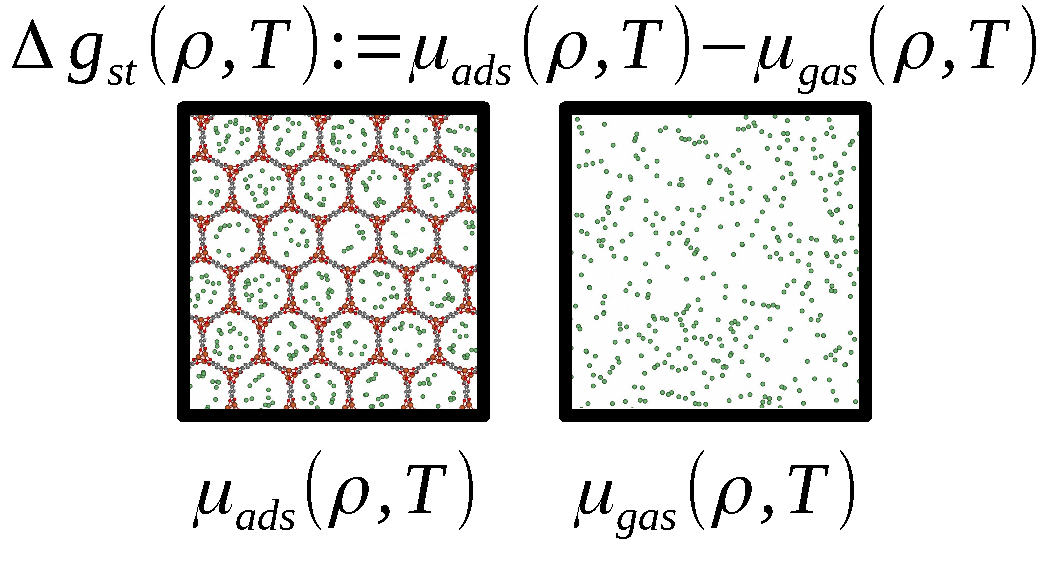
\includegraphics[width=\columnwidth]{g_st_simple.pdf}
    \caption{Cartoon illustrating the definition of $\gst$. for a given adsorbent and gas, $\gst$=$\gst (\rho, T)$ is defined as the difference in chemical potential between the adsorbed gas system and bulk gas system when both exhibit the same density and temperature.}
    \label{fig:delta-G-cartoon}
\end{figure}

The parameter describing our idealized substrate is $\V$, the spatially uniform
potential felt by a gas molecule adsorbed in the idealized substrate. A natural
question is how this potential relates to the properties of real substrates.
The effect of $\V$ in our model is to shift the chemical potential $\mu$ of the
gas (see Sec.~\ref{sec:V_shifts_chem_pot}). Because our ideal substrate shifts
the chemical potential of the gas molecules by providing a spatially uniform
potential energy field, the entropy of the gas in the ideal substrate is equal
to the entropy of the gas in its bulk state at the same density and
temperature. In contrast, a real substrate provides a non-spatially uniform
potential. Consequently, the entropy of the gas inside a real substrate is
\emph{not} equal to the entropy of the bulk gas at the same density and
temperature. Therefore, the parameter analogous to $\V$ in a real substrate
will involve both energy and entropy. The real-substrate analog of $\V$ is the
shift of molar Gibbs free energy provided by the substrate, specifically an
\emph{isosteric} (or constant-density) shift of the Gibbs free energy:

\begin{equation}
   \gst(\rho, T) \equiv
   %\frac{G_{\text{ads}}(\rho, T) - G_{\text{gas}}(\rho, T)}{N}\\
    \mu_{\text{ads}}(\rho, T) - \mu_{\text{gas}}(\rho, T).
  % \gst(\rho, T) &\equiv g_{\text{gas}}(\rho, T) - g_{\text{ads}}(\rho, T)
  \label{eq:g_st}
\end{equation}
The isosteric Gibbs free energy difference $\gst$ is the difference in molar
Gibbs free energy (equivalent to chemical potential) between the adsorbed gas system and
the bulk gas \emph{with the same density of gas molecules}. The quantity $\gst$
does \emph{not} correspond to a change in the molar Gibbs free energy as a
molecule is adsorbed, which is zero under conditions of coexistence. The
quantity $\gst$ in a real substrate is a direct analog to $\V$ in our ideal
substrate because it is the chemical potential shift needed to impose on the
bulk gas in coexistence with the real substrate to achieve the same density as
in the substrate (compare with eqn.~\ref{eq:xi_vs_xi0}).
Figure~\ref{fig:delta-G-cartoon} illustrates a hypothetical experiment to
measure $\gst$ via a piston with a removable partition that separates a volume
of free space from the same volume of substrate. Note that $\gst$ is a property
of both the substrate and the identity of the gas. Because real substrates
offer a \emph{non}-spatially uniform potential, $\gst(\rho, T)$ is a function
of $\rho$ and $T$, unlike our ideal, homogenous substrate where $\gst(\rho,
T)=\V$. Consequently, throughout this article, we show $\gst(\rho, T)$ for real
substrates at both conditions relevant to gas storage and delivery, $\pfull$
and $\pempty$.

In practice, we can readily compute $\gst(\rho, T)$ of a real gas/substrate
system from (i) the (experimental or simulated) equilibrium adsorption isotherm
of the gas in the substrate and (ii) the (experimental or simulated) chemical
potential of the bulk gas. Consider the real substrate in thermodynamic
equilibrium with a bulk gas at fixed temperature $T$ and pressure $p$, and let
$\rho=\rho(p, T)$ be the density of gas in the substrate. At coexistence, the
chemical potential of the bulk gas is equal to the chemical potential of the
adsorbed gas in the substrate. Thus, we can use the experimentally known molar
Gibbs free energy of the pure, bulk gas system at temperature $T$ and pressure
$p$ to determine the molar Gibbs free energy of the adsorbed system:
$\mu_{\text{ads}}(\rho, T)=\mu_{\text{gas}}(p, T)$. We can then also look up
the known chemical potential of the bulk gas at the same density and
temperature as in the substrate, $\mu_{\text{gas}}(\rho, T)$. Via
eqn.~\ref{eq:g_st}, $\gst$ follows from subtracting the two quantities.

An interesting question is how $\gst$ relates to the commonly measured and
reported isosteric heat of adsorption $q_{st}$, which is roughly the energy
change when a gas molecule is adsorbed~\cite{sircar1999isosteric,
tian2017differential}. Figure~\ref{fig:qst-vs-delta-G} shows how $q_{st}$
compares to $\gst$ for several prominent adsorbents. In every case,
$|q_{st}|>|\gst|$ because the gas in the adsorbent always has less entropy than
the gas in the bulk at the same density and temperature. That is, while
adsorption is energetically favored, it is entropically disfavored due to the
restrictions imposed on the configuration of the gas molecules via steric
interactions with the substrate itself; this counters the energetic attraction.

\begin{figure}
    \centering
    \includegraphics[width=0.95\columnwidth]{qst-vs-delta-G}
    \caption{Relationship between $\gst$ and the isosteric heat
      $q_{st}$ for several prominent adsorbents at room
      temperature (data from Ref.~\cite{mason2014evaluating, garcia2018benchmark}). The dots represent the properties of methane
      adsorption at 5.8~bar and 65~bar. The $+$'s represent the
      properties of hydrogen adsorption at 5~bar and
      100~bar.}
    \label{fig:qst-vs-delta-G}
\end{figure}

\begin{figure}
    \centering
    \includegraphics[width=0.95\columnwidth]{methane-298-gst}
    \caption{The density-dependence of $\gst$ of methane in several
      adsorbents (298\ K). Note that $\gst$ is monotonic in
      $\rho$. Data from
      Refs.~\cite{mason2014evaluating, furukawa2009storage}.
    }
    \label{fig:methane-gst}
\end{figure}

\begin{figure}
\centering
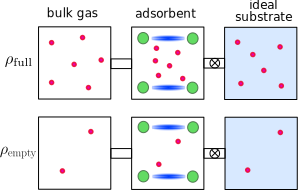
\includegraphics[width=0.95\columnwidth]{four-cases-pro}
\caption{Two pairs of two connected and equal volumes containing gas. In the top pair, the density of gas in each volume is $\rhofull$. In the bottom pair, the density of gas in each volume is $\rhoempty$. The two volumes on the left are packed with a porous material. The two volumes on the right offer a spatially uniform background potential energy $\V$ (our idealized substrate). A connection between the two volumes in each pair has a valve to allow flow of gas between them}
\label{fig:delta-gst-maximum}
\end{figure}

\section{An upper bound when $\gst(\rho)$ is monotonic}\label{sec:monotonic}
Every MOF has a $\Delta g_\text{st}$ at $\pfull$ and $\pempty$ corresponding
to a full and empty density. The deliverable capacity of the MOF is equal to
the difference between the full and empty density. Examining
Fig.~\ref{fig:methane-gst}, we see that a significant variety of known
experimental $\Delta g_\text{st}$ curves are monotonic. Furthermore, our
qualitative argument in Section~\ref{sec:upper-bound} suggests that this
function \emph{should} monotonically increase for rigid substrates, as
increasing the density of gas causes some of the gas to reside in higher-energy
sites. If this is always the case, the deliverable capacity of a real material
(with a non-spatially uniform potential) with a given $\gst$ at $\pfull$ or
$\pempty$ is bounded below by the deliverable capacity in our idealized
substrate with $\V=\gst$, even for a value of $\V$ that is not optimal.

To show this, we perform a thought experiment illustrated in
Fig.~\ref{fig:delta-gst-maximum}. We begin with two pairs of volumes.  Two of
these volumes contain a real adsorbent material.  These adsorbent volumes are
connected to bulk gas reservoirs at $\pfull$ and $\pempty$ respectively, and
therefore have densities $\rhofull$ and $\rhoempty$.  The other two volumes
volumes have equal density to the two adsorbent volumes ($\rhofull$ and $\rhoempty$), but contain our
idealized substrate with uniform potential energy $\V$.

We now consider what happens if we open a diffusive connection between a
volume of MOF and a volume with an idealized substrate that initially contain
the same density of gas, for instance by connecting them with a tube. If the
chemical potential in the idealized substrate is higher than in the porous material,
then gas will flow out of the idealized substrate, lowering its density.  Conversely
if the chemical potential is lower in the idealized substrate than in the
volume of porous material, then gas will flow into the idealized substrate, increasing
its density.
The difference in chemical potential between those two volumes is
\begin{align}
   \gst(\rho) - \V &= \left(\mu_{\text{MOF}}(\rho) - \mu_{\text{gas}}(\rho)\right)
   - \left(\mu_{\V}(\rho) - \mu_{\text{gas}}(\rho)\right)
   \\
   &= \mu_{\text{MOF}}(\rho) - \mu_{\V}(\rho).
\end{align}
where $\mu_{\text{MOF}}(\rho)$ and $\mu_{\V}(\rho)$ are the chemical potentials
of gas in the porous material and ideal substrate with potential $\V$, respectively.
Thus if $\gst(\rhoempty) =
\V$ then the low-density containers will remain at their initial density after
they are connected. Thus, the deliverable capacity of the MOF will be greater
than the deliverable capacity of the ideal substrate with uniform potential $\V$ if and
only if $\gst(\rhofull)<\V$, i.e. if $\gst(\rho)$ does \emph{not} monotonically
increase, since the gas in the high-density system will flow from the ideal
substrate to the MOF. By the same token, if we consider the case where
$\gst(\rhofull) = \V$, then for the MOF to achieve a greater deliverable
capacity than the idealized substrate, the MOF must have less residual gas,
which means that gas must spontaneously flow from the low-density MOF to the
volume with potential $\V$, which means that $\gst(\rhoempty)>\V$. Once again,
exceeding our upper bound requires a material with a $\gst(\rho)$ that does not
increase monotonically.

Taken together, this indicates that not only is our absolute upper bound an
upper bound for rigid MOFs, but the green curve labeled $\rho_D(\gst)$ in
Figs.~\ref{fig:methane-298-D}, \ref{fig:hydrogen-298-D}, and
\ref{fig:hydrogen-77-D} is an upper bound for materials with a non-optimal
$\gst$ at either $\pfull$ or $\pempty$.

\section{Cryogenic hydrogen storage}\label{sec:cryo-hydrogen}
\begin{figure}
    \centering
    \includegraphics[width=0.95\columnwidth]{hydrogen-77-n-vs-G}
    \caption{Deliverable capacity of hydrogen at 77\ K as a function of the attractive Gibbs free energy $\gst$. Experimental deliverable capacities for several porous materials (data from Ref.~\cite{garcia2018benchmark}) are shown along with the experimental values for $\gst$ at the empty and full pressures shown as $+$'s connected by a line.}
    \label{fig:hydrogen-77-D}
\end{figure}

One approach to increase the deliverable capacity is to reduce the storage
temperature. This is illustrated in Fig.~\ref{fig:hydrogen-77-D}, which shows
the upper bound to the deliverable capacity of hydrogen at 77\ K, the boiling
point of nitrogen. The DOE ULTIMATE target in this case looks far more
achievable, and with a much lower $|\gst|$. In fact, an empty tank at this
temperature can satisfy the DOE 2020 target. The DOE ULTIMATE target is 14\%
below the upper bound. Actual MOFs fall far short of the theoretical maximum.

\end{document}